As is oftentimes the case when aiming to model realisitic physical systems, the equations of motion presented here do not admit closed-form analytical solutions. As such, we must rely on numerical methods and computer simulations to solve them. Specifically, we solve $N$ independent sets of Hamilton's equations, each consisting of six first-order, coupled differential equations.

Numerical integration presents several challenges. First, there is the practical question: how do we actually solve these equations? Most students first encounter a simple update scheme, such as Euler's method: $y_{i+1} = y_i + \frac{dy}{dt}\Delta t$. However, this quickly becomes insufficient for coupled systems or for problems where precision and conservation laws are essential. How can we be confident that our numerical solutions faithfully approximate the true dynamics, especially when the true solution is unknown? How do we handle performance, data volume, or the trade-offs between speed and accuracy?

Although many software packages already exist to solve such problems, I chose to write my own code. This led to the development of \texttt{tstrippy}, a code designed to solve the restricted three-body problem. My motivation was part practical: I wanted to avoid installation difficulties, steep learning curves, and uncertainty over whether existing tools could handle my specific setup. But above all else, I wanted to create a reliable product that works, allows me to reproduce my results, and run my simulations at scale. 

Developing my own package gave me a deeper understanding of code structure, numerical algorithms, and the subtleties of scientific programming. It also gave me the confidence to later use other packages more effectively. The \texttt{tstrippy} code is available on GitHub and runs on macOS and Linux.

This chapter documents how I numerically solve the equations of motion, how I validate the accuracy of the solutions, and how the code is organized under the hood.



\section{Astronomical units and scaling}

    When writing any code, the choice of units is important. Astronomical units are rarely the same as SI units. In general, the choice of units is observationally and historically motivated, resulting in a system that uses multiple units for the same physical quantity, which can be confusing at first.

    For instance, sky positions are typically reported in spherical coordinates. Right ascension (analogous to longitude) is often expressed in either degrees or hours, while declination (similar to latitude) is given in degrees. Distances are reported in parsecs when derived from parallax measurements. Line-of-sight velocities, obtained via spectroscopic Doppler shifts, are reported in kilometers per second. Proper motions describe angular displacements over time on the sky  and are usually reported in milliarcseconds per year. Already, we encounter several different units for angles (degrees, hours, arcseconds), time (years, seconds), and distance (km, kpc), none of which align with SI’s standard units of radians, seconds, or meters, as summarized in Table~\ref{tab:units}.

    \begin{table}[]
        \caption{Units for various astronomical quantities in Galactic and SI systems.}
        \label{tab:units}
        \begin{tabular}{l|l|l|l|l|l|l|}
                            & Distance  & RA                     & DEC                    & \textbf{$\mathrm{v}_\mathrm{LOS}$} & $\mu_\alpha$ & $\mu_\delta$ \\ \hline
            Galactic: & {[}kpc{]} & {[}deg{]} {[}HHMMSS{]} & {[}deg{]}              & km/s                      & {[}mas/yr{]} & {[}mas/yr{]} \\ \hline
            S.I.       & {[}m{]}   & {[}rad{]}              & {[}rad{]}              & m/s                       & {[}rad/s{]}  & {[}rad/s{]}  \\ 
        \end{tabular}
    \end{table}

    This raises practical concerns—for example, what would be the unit of acceleration? km/s$^2$? parsec/year/second? To systematically manage units, we turn to dimensional analysis, notably the Buckingham Pi theorem \parencite{1914PhRv....4..345B}. In classical mechanics, physical quantities are typically expressed in terms of three fundamental dimensions: length, time, and mass. Any quantity can then be represented as a product of powers of these base units:

    \begin{equation}
        \left[\mathrm{Quantity}\right] = l^a t^b m^c =
            \begin{bmatrix}
                a\\
                b\\
                c 
            \end{bmatrix}
    \end{equation}

    For example, velocity has dimensions $[1, -1, 0]$, momentum is $[1, -1, 1]$, and acceleration is $[1, -2, 0]$.

    It is not strictly necessary to adopt length-time-mass as the fundamental basis, as long as the three chosen base units are linearly independent. In stellar dynamics, it is often more natural to use distance, velocity, and mass as the base units. In this thesis, I adopt:
    \begin{itemize}
        \item Distance: 1~kpc
        \item Velocity: 1~km/s 
        \item Mass: 1~solar mass $\mathrm{M}_\odot$
    \end{itemize}

    In this system, time has derived units of:
    \begin{equation}
        \left[t\right] = \frac{\mathrm{distance}}{\mathrm{velocity}} = \frac{\mathrm{kpc}}{\mathrm{km/s}}.
    \end{equation}
    While not immediately intuitive, this unit of time is convenient because:
    \begin{equation}
        1\frac{\mathrm{kpc}}{\mathrm{Gyr}} \approx 1\frac{\mathrm{km}}{\mathrm{s}}.
    \end{equation}

    The gravitational constant has dimensions:
    \begin{equation}    
        \left[G\right]=\frac{v^2 \cdot l}{m},
    \end{equation} 
    which evaluates numerically in these units as: 
    \begin{equation}
        G = 4.301 \times 10^{-6} \left(\mathrm{km}/\mathrm{s}\right)^2 \cdot \mathrm{kpc} \cdot \mathrm{M}_\odot^{-1}.
    \end{equation}

    Once the base units are defined, derived quantities such as acceleration follow directly. Whether considering acceleration as $v^2~l^{-1}$ or $l \cdot t^{-2}$, they are equivalent and yield: $\left(\mathrm{kpc}/\mathrm{s}\right)^2 \cdot \mathrm{kpc}^{-1}$.

    It is worth mentioning that $N$-body codes often select distance, velocity, and the gravitational constant as the base units, setting $G = 1$. While this choice simplifies force computations, it introduces less intuitive units for mass. For instance, by choosing 1~kpc for distance and 1~km/s for velocity, and setting $G = 1$, the derived mass unit becomes:
    \begin{equation}
        \left[\mathrm{mass}\right] = \frac{l \cdot v^2}{G} = 232509~\mathrm{M}_\odot.
    \end{equation} This approach was used in our first paper (see Chapter~4). 
    
    Another example is the case of \texttt{Galpy}. \citet{2015ApJS..216...29B} introduced \textit{natural units} motivated by the galaxy's rotation curve, embodied in:

    Another possibility is to choose \textit{natural} units, as done by \citet{2015ApJS..216...29B} in \texttt{Galpy}. More specifically, \citet{2015ApJS..216...29B} uses a normalization in which $R$, the cylindrical scale length of the galaxy, and $v_\mathrm{circ}$, the circular velocity at this radius, are both set to 1. This choice is motivated by a galaxy's rotation curve and is embodied in:
    \begin{equation}
        \frac{v_\mathrm{circ}^2}{R_0} = \nabla  \Phi \left(R_0, z=0\right).
        \label{eq:vcirc}
    \end{equation}
   Note that the gravitational constant is also set to 1. Whatever the form of the potential, the scale lengths must be normalized to $R$, and the mass parameter is subsequently determined through Eq.~\ref{eq:vcirc}. The total potential is a linear combination of individual components, with the user selecting the contribution of each component to the force at the characteristic radius. For example, $\Phi = \sum_i a_i\Phi_i$, where $a_i$ are weights such that $\nabla \Phi_i(R_0, z=0) = a_i$ in normalized units. In this system of units, emphasis is placed on the rotation curve and how much each component contributes to it at the reference radius of the galaxy. Note that $v_\mathrm{circ}(R_0)$ is not necessarily the maximum value of the rotation curve.

    In short, each code presents its own preferred units and normalization. \texttt{Tstrippy}, by contrast, expects the user to pass masses in solar masses, velocities in kilometers per second, and distances in kiloparsecs. However, physical constants are not hard-coded, so the user may pass any numerical values to the code as long as they are based on a self-consistent unit system. Despite this, the code comes equipped with parameters for the \texttt{Pouliasis2017pii} potential and for the catalog of globular clusters. These values are reported in the aforementioned units.

    A valid general strategy when developing numerical codes is to implement a module that converts user-defined units to the internal units of the code. This functionality also exists in \texttt{Galpy} and a similar system is implemented in \texttt{Agama} \citep{2018arXiv180208255V}. I chose not to add such a layer to \texttt{Tstrippy} since \texttt{Astropy} provides an excellent unit-handling module that allows users to convert between units easily \citep{2013A&A...558A..33A}, and I recommend its use in the documentation. 



\section{Solving the equations of motion}

    Long before the advent of computers, Euler proposed (1707-1783) a simple method for numerically solving differential equations. In this method, a solution is found by: 
    \begin{equation}
        y_{i+1} = y_i + \Delta t \frac{dy}{dt}\left(y,t\right),
    \end{equation}
    where $i$ is an index. This means that at each point $(t_i,y_i)$, the function is extrapolated to obtain the next position with a simple linear approximation. This has very limited accuracy and can be shown by considering taylor series expansion about $y_{i+1}=y\left(t_i+\Delta t\right)$. With a Taylor series, we could approximate the function to infinitely many terms:
    \begin{equation}
        y\left(t_i+\Delta t\right) \approx y(t_i) + \Delta t y'(t_i) + \frac{1}{2!}\Delta t^2 y''\left(t_i\right) \dots
    \end{equation}
    and the difference between the true solution and numerical solution found through Euleur's method are all the terms that are higher order than the linear term.  When describing the accuracy of the numerical soluition to the true solution, we use the Big-O notation, whose argument is the leading order term that drives the inaccuracy. For Euler's method, the accuracy is of a single step is dictated by the second order term: $\mathrm{Err}_\mathrm{step} \approx  \Delta t^2 \frac{1}{2!} y''\left(t_i\right)$, which in Big-O notation is $\mathcal{O}\left(\Delta t^2\right)$. Overall, if we quantify the accuracy of the solution, it would be the number of steps times the average error per step: $\mathrm{Err} \approx N_\mathrm{step} \langle \mathrm{Err}_\mathrm{step} \rangle$, which becomes: $\mathrm{Err} \approx \frac{T}{\Delta t} \times \Delta t^2\langle y''\rangle$. For the whole solution, the error is linearly propertional to the timestep: $\mathcal{O}\left(\Delta t\right)$. This notation reads as halfing the timestep halfs the error. 
    
    Note that this method for quantifying the error is of a numerical solution is not mathematically rigorous and nor generalizable. The amount of error accumulated throughought the integration depends on the function. For instance, if the $y$ is linear equation, and $y'$ is constant, than there is no error with Euler's method. If $y$ a simple power of $t$, $y=t^a$, then the errors will always accumulate and grow monotonically. If $y$'s concavity and curvature change as a function of $t$, the error between two adjacent steps could cancel each other out. 
    
    Chapter 16 in Numerical Recipe's in C presents an excellent introduction to this problem and provides many alternatives to Euler's method \parencite{1992nrca.book.....P}. The point remains, that in any case, one must perform sanity checks to ensure themselves that a proper solution has been reached that only deviates from the true solution by a tolerable amount. These test could include exploring different integration scheme's, convergence testing, that the solution converges as the timestep is reduce, and also exploiting any other known properties about your solution.  

    In the case of Hamiltonian systems, we can exploit specific geometric properties to design numerical schemes that better preserve the qualitative features of the true solution.

    In this thesis, I implemented the Leapfrog integrator and the Forest-Ruth scheme. These schemes are derived from the structure of Hamiltonian mechanics and are known as \textit{symplectic integrators}. Before continuing, I would like to quote \citep{bovy_inprep}:

    \begin{quote}
        Hamiltonian integrators are often called symplectic. This name comes from the fact that these integrators are Hamiltonian maps, whose mathematical structure is that of a vector flow on a symplectic manifold. Many fine dynamicists have made great contributions to the field without delving deeply into the meaning of the previous sentence and we do not discuss this further.
    \end{quote}

    However, my curiosity about linguistics pushed me to delve further: What does \textit{symplectic} mean? \citet{weyl1946classical} coined the term because \textit{complex} was already taken. The prefix \textit{com} refers to together, and ``plexus'' comes from greek meaning ``woven'' or ``braided''. So from its roots, “complex” means something composed of interwoven parts. The image of tangled braids captures the idea well. Similarly, ``sym-'' is a Greek prefix meaning “together.” The idea remains the same: in Hamiltonian dynamics, the evolution of position and momentum are interdependent. This becomes clearer in matrix form:
    \begin{equation}
        \begin{bmatrix}
            \dot{\bf{q}}\\
            \dot{\bf{p}}
        \end{bmatrix}
         = 
        \begin{bmatrix}
            0 & I_n \\
            -I_n & 0 
        \end{bmatrix}
                \begin{bmatrix}
            \frac{\partial \mathcal{H}}{\partial \bf{q}} \\
            \frac{\partial \mathcal{H}}{\partial \bf{p}}
        \end{bmatrix}
        \label{eq:symplectic}
    \end{equation}
    Here, the skew-symmetric matrix “weaves” the positions and momenta together.

    Although the equations of motion do not admit analytical solutions, they possess several known properties. First, trajectories governed solely by gravity are time-reversible. This property is important for my methodology, where I integrate the equations of motion backward in time and then forward again to the present-day position. Secondly, the total orbital energy is conserved. Moreover, according to Liouville's theorem, Hamiltonian flows preserve the local phase space volume. A corollary of this is that the determinant of the Jacobian matrix of the transformation from $\left(q,p\right)\rightarrow \left(q',p'\right)$ must be one, which means that the transformation only rotates or translates an infinitesimal volume but does not shrink or expand the volume. We can view the transform as: 
    \begin{eqnarray}
        q' &= q + \frac{\partial \mathcal{H}}{\partial p}\Delta t, \\
        p' &= -\frac{\partial \mathcal{H}}{\partial q}\Delta t + p,
    \end{eqnarray}
    The Jacobian matrix is given by $\left(\frac{\partial x_i'}{\partial x_j }\right)$: 
    \begin{equation}
        \begin{bmatrix}
            1 & \Delta t \frac{\partial^2 \mathcal{H}}{\partial p^2} \\  
            -\Delta t \frac{\partial^2 \mathcal{H}}{\partial q^2} & 1 \\  
        \end{bmatrix}
    \end{equation}
    and the subsequent determinant is: 
    \begin{equation}
        \mathrm{det}\left(J\right) = 1 - \Delta t^2 \frac{\partial^2 \mathcal{H}}{\partial q^2} \frac{\partial^2 \mathcal{H}}{\partial p^2}.
    \end{equation}
    In general, neither $\frac{\partial^2 \mathcal{H}}{\partial q^2}$ or $\frac{\partial^2 \mathcal{H}}{\partial p^2}$ are zero. Therefore, to preserve phase-space volume, we update positions and momenta in alternating steps. The transformation order becomes: $(q,p) \rightarrow (q',p) \rightarrow (q',p')$. This is commonly referred to as a sequence of \textit{drifts} and \textit{kicks}. A \textit{drift} updates the position while holding the momentum fixed, and a \textit{kick} updates the momentum while holding the position fixed. Symplectic integrators alternate these operations in a specific sequence to preserve the structure of Hamiltonian flow.

    The scheme outlined above is essentially a first-order method and is closely related to Euler's method. More sophisticated integrators use values from multiple time steps to construct higher-order estimates of the system's evolution. For example, some schemes temporarily evolve the position to an intermediate value $q_\mathrm{temp}$, use this to compute a momentum $p_\mathrm{temp}$, and then adjust both using weighted averages or predictor-corrector steps to reach the final state. These methods carefully balance forward and backward steps to optimize accuracy while preserving the symplectic structure.

    One of the most commonly used integrators in galactic dynamics is the leapfrog method. It works by interleaving updates of positions and momenta using time-centered averages. Specifically, the average momentum between $q_i$ and $q_{i+1}$ (denoted $p_{i+1/2}$) is used to advance the position, and then the average force (derived from the potential) is used to update the momentum. In Cartesian coordinates—used throughout this thesis—the leapfrog algorithm can be written as:


    \begin{eqnarray}
        x_{i+1/2} &= x_i + \frac{1}{2} \dot{x}_i \Delta t , \\
        \ddot{x} &= -\nabla \Phi(x_{i+1/2}), \\
        \dot{x}_{i+1} &= \dot{x}_i + \ddot{x} \Delta t, \\
        x_{i+1} &= x_{i+1/2} + \frac{1}{2} \dot{x}_{i+1} \Delta t. \\
    \end{eqnarray}
    As I will show in the next section, the leapfrog algorithm is sufficient for the problems that I solve. However, the question of computational efficiency and numerical accuracy is ever present. Leapfrog uses uses the two local points about the position and momenta to evolve them. Other schema can use more points to have more accurate estimations for the local derivatives. 
    
    \citet{1990PhyD...43..105F} proposed one such method for symplectic integrations, which is our situation here. The method is complicated and involves finding roots of high order polynomials, and the roots of which determine the weights and distances about the local point for finding the best estimate of the derivative for evoling the system. The method involves solving a cubic polynomial to determine the optimal coefficients. While the derivation is mathematically involved, the final scheme is straightforward to implement. Nonetheless, I implemented this method and tested its efficiency against the leapfrog. There are eight coefficients in this method, which are presented in table~\ref{tab:forest_ruth_coeffs}.
    \begin{table}[h]
        \centering
        \caption{Velocity (\(c_n\)) and acceleration (\(d_n\)) coefficients for the Forest-Ruth symplectic integrator.}
        \label{tab:forest_ruth_coeffs}
        \begin{tabular}{ccccc|cccc}
            \multicolumn{4}{c|}{Velocity coefficients (\(c_n\))} & \multicolumn{4}{c}{Acceleration coefficients (\(d_n\))} \\
            $c_1$ & $c_2$ & $c_3$ & $c_4$ & $d_1$ & $d_2$ & $d_3$ & $d_4$ \\
            \hline
            $w + \frac{1}{2}$ & $-w$ & $-w$ & $w + \frac{1}{2}$ & $2w + 1$ & $-4w - 1$ & $2w + 1$ & $0$ \\
        \end{tabular}
    \end{table} 
    The coefficients are all based on the solution to the cubic polynomial: $48 w^3 + 24 w^2 - 1 = 0 $. For a single step, the positions and velocities are updated as follows:
    \begin{align} 
        x' &= x + c_n v \Delta t \\ 
        t' &= t + c_n \Delta t \\ 
        \ddot{x} &= \nabla \Phi (x') \\ 
        \dot{x}' &= \dot{x} + d_n \ddot{x} \Delta t,
    \end{align}
    where $n$ is the \textit{mini-step}. Notice that the sum of $\sum_n^4 c_n$ and $\sum_n^4 d_n$ both equal 1, which is a full time step $\Delta t$. 

    Lastly, it is important to note that the leapfrog algorithm is symplectic and time-reversible only for Hamiltonians that are both time-independent and separable—that is, where the Hamiltonian can be written as a sum of a kinetic term depending only on momenta, $T(p)$ and whose potential depends only on position $\Phi(q)$. These conditions are satisfied for systems in an inertial frame with conservative forces. This is true when I integrate the motion for the center of mass of the globular clusters. However, the Hamiltonian for the integration of the particles does depend on time. So the leapfrog algorithm may introduce systematic integration errors due to the violation of its underlying assumptions, beyond ordinary rounding errors.

    Similarly, when we integrate the orbits of either the particles or the globular clusters in the galaxy containing a galactic bar, we are faced with a choice: we can either work in a time-dependent inertial frame, where the potential rotates and the Hamiltonian explicitly depends on time, or we can transform to a rotating frame, in which case the kinetic energy becomes position-dependent due to Coriolis and centrifugal forces, which breaks the necessary criteron of separability: $\mathcal{H}(q,p) = T(p)+\Phi(q)$. In both cases, the standard assumptions of the leapfrog algorithm are violated.

    Nonetheless, we will continue to use leapfrog as it remains a robust and efficient integrator for a wide range of astrophysical systems. Its good long-term energy behavior makes it a reasonable approximation even when the ideal assumptions are not strictly met. However, this highlights the need for careful validation: we must verify that the integration errors remain within acceptable bounds, especially in systems with non-separable or time-dependent dynamics. This validation is the subject of the next section.


\section{Numerical Error \& Computation Time}

    To ensure the quality of the integration, I perform two main checks. The first is to ensure that the initial orbital energy of a given particle is conserved to high precision. At each timestep, the relative error in the energy conservation is: $
    \mathrm{err}(E_i) = \left|\frac{E_i - E_0}{E_0}\right|$, where $E_0$ is the initial energy and $E_i$ is the orbital energy at the index for a given time step $i$. For the case of just globular clusters, the orbital energy it's own kinetic energy plus it's gravitational potential energy in galaxy: $E_i = T(\textbf{v}_i) + \Phi_{\mathrm{MW}}\left(\textbf{x}_i\right)$. For the case of a star-particle within a globular cluster, the potential energy of the cluster is included: $E_i = T(\textbf{v}_i) + \Phi_{\mathrm{MW}}\left(\textbf{x}_i\right) + \Phi_\mathrm{GC}\left(\textbf{x}_i - \textbf{x}_{\mathrm{GC},i}\right)$. The same goes for the potential with the galactic bar, the only difference being that potential has a time-dependent element. 

    The second check is that simulations are time-reversable. In this case, I integrate a cluster back in time by a given amount of time, and then change the sign of its velocity to subsequently integrate forward in time. If the integration is correct, the cluster should remain on the same trajectory. I investigate this for four scenarios and show the results below: 
    \begin{itemize}
        \item The globular cluster population orbiting with a time-static Milky Way potential;
        \item Star-particles orbiting with a stationary and isolated globular cluster;
        \item Full stream generation, i.e., star particles orbiting within a globular cluster that orbits the galaxy,
        \item The globular clusters orbiting in a potential with a galactic bar; 
        \item Star-particles orbiting within a globular cluster in a Milky Way with a Galactic bar.
    \end{itemize}

    \subsection{Globular Cluster Orbits in a Static Galaxy}

        As explained in the next chapter, the initial conditions for the globular cluster system (positions and velocities), were taken from \citet{2018MNRAS.478.1520B}'s online globular cluster catalog whose data derived from Gaia Early Data Release 3 among other sources \citep{2021MNRAS.505.5957B,2021A&A...649A...1G,2023A&A...674A...1G}. 

        To test the integrator, I integrated the whole globular cluster system for 5~Gyr, and then integrated it back to the initial conditions. I used four time steps: $10^4,10^5,10^6,10^7$~years which corresponds to $\left[500,5000,50000,500000\right]$ integration steps, respectively. In general, the time step should scale with the dynamical time of the orbit, or be inversely proprotial to the orbital energy. The farther the system is from the center, a large time step could be sufficient for low numerical error. However, those who complete many orbits should have a smaller timesteps. Of course, it does not scale with just orbital energy, it should scale with the maximum acceleration experienced in the system. A highly eccentric orbit requires a smaller timestep to properly integrate the motion near the pericenter, compared to a circular orbit at the same orbital energy. To not clutter the graph, in Fig.~\ref{fig:numericalErrorLeapFrogVanilla}, I present the whole globular cluster system twice each integrated with the smallest and largest timesteps: $10^4$ and $10^7$ years. 

        \begin{figure}
            \centering
            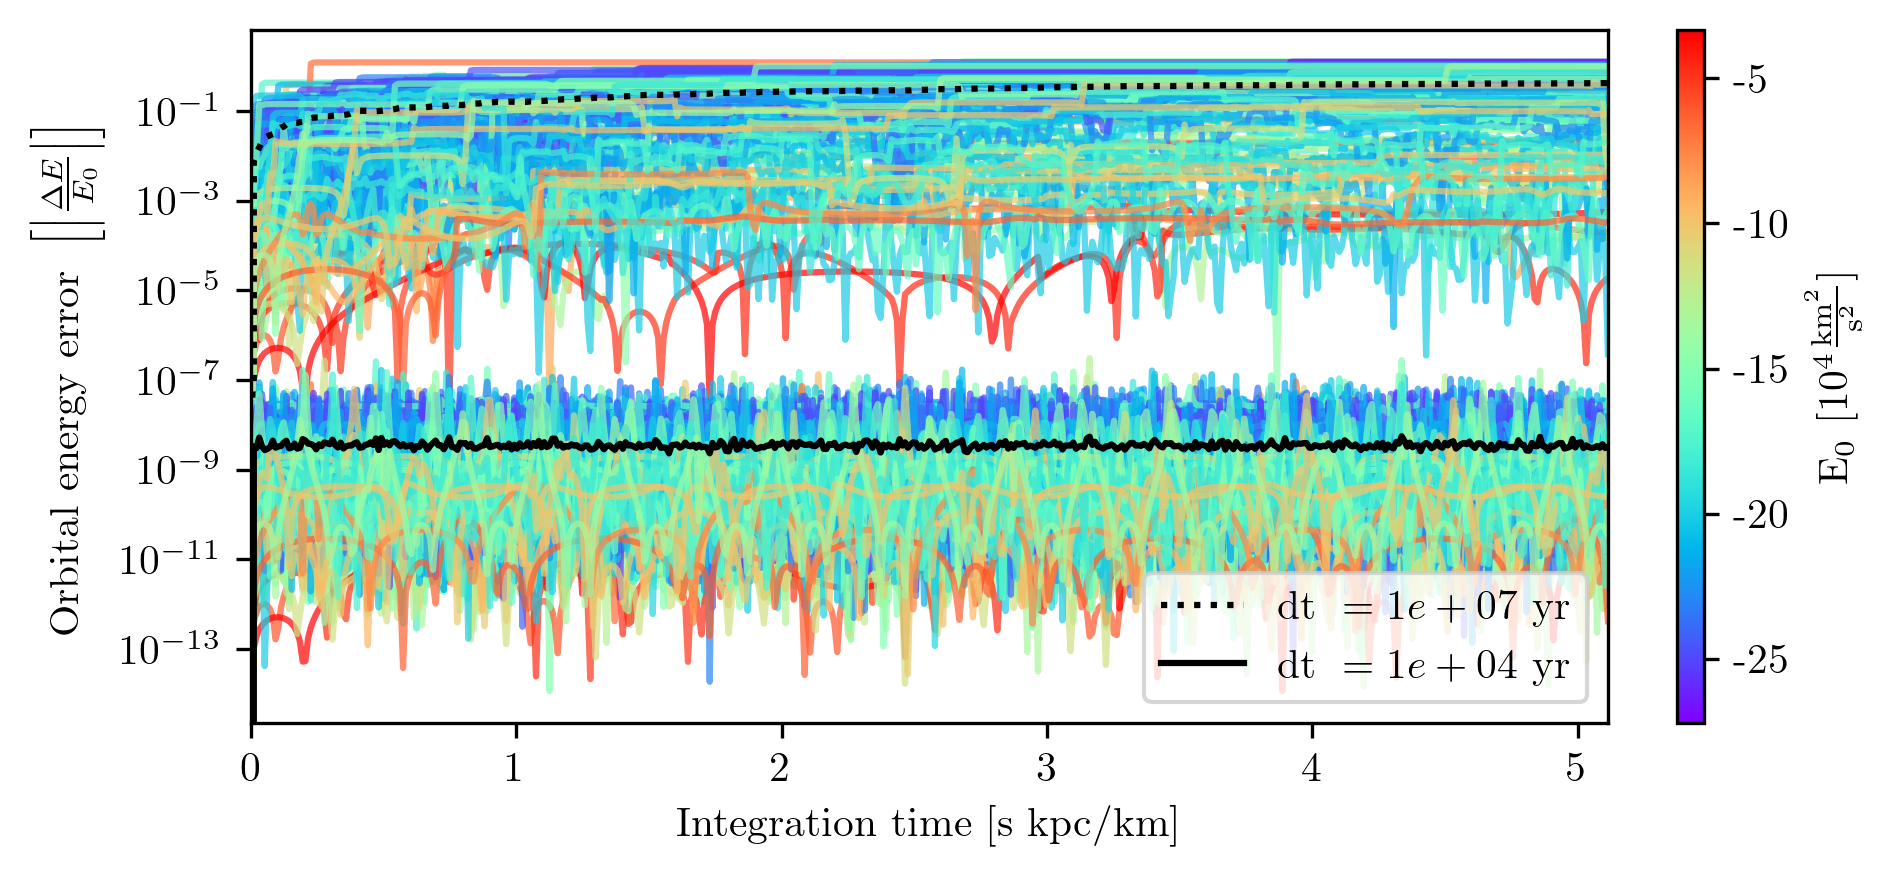
\includegraphics[width=\linewidth]{images/numericalErrorLeapFrogVanilla.png}
            \caption{Error in orbital energy for the whole globular cluster system with two different time steps, dt~=~$10^{7}$ and $10^{4}$ years. Each cluster's is colored by it's initial orbital energy. The average of the whole system for a given timestep is indicated with dotted and solid black lines. }
            \label{fig:numericalErrorLeapFrogVanilla}
        \end{figure}
        In Fig.~\ref{fig:numericalErrorLeapFrogVanilla} we can notice that orbits with higher orbital energy in red have low numerical error compared to those with lower energy and are deeper in the potential well. It is clear that for the whole system, $10^7$~years is a time step that is far too large, however, interestingly enough, for some of the farthest globular clusters, a time step of 10 million years resolves their orbits to an error of $\langle \Delta E / E_0 \rangle \sim 10^{-5}$, which is still far less than the uncertainties in the energy due to both modeling and observational uncertainties.
    

        In Fig.~\ref{fig:numericalErrorReverseIntegration}, I present the \textit{time reversibility}, or the integrator's ability to retrace it's own steps. For each given time step, I report the difference between the initial integration and the retrace normalized to the mean of the two position's. I perform the same computation for the velocities. The time step of $10^7$~yr saturates only after 2~Gyr. The distances do not continue to grow becuase the orbital energy only differs by one part in ten, so at later time steps, the cluster is still within the same region of phase-space, but the retrace is at a completely different location than the initial integration. The errors in the time step of $10^6$~yrbecome significant, though by the end of the integration period of 5~Gyr they are still only one part in ten thousand. The time steps of $10^5$ and $10^4$~yr have excellent retraceability and on average, only differ by one part in $10^{-14}$, and are thus only limited by round off error from the use of double precision floating point numbers.
        \begin{figure}
            \centering
            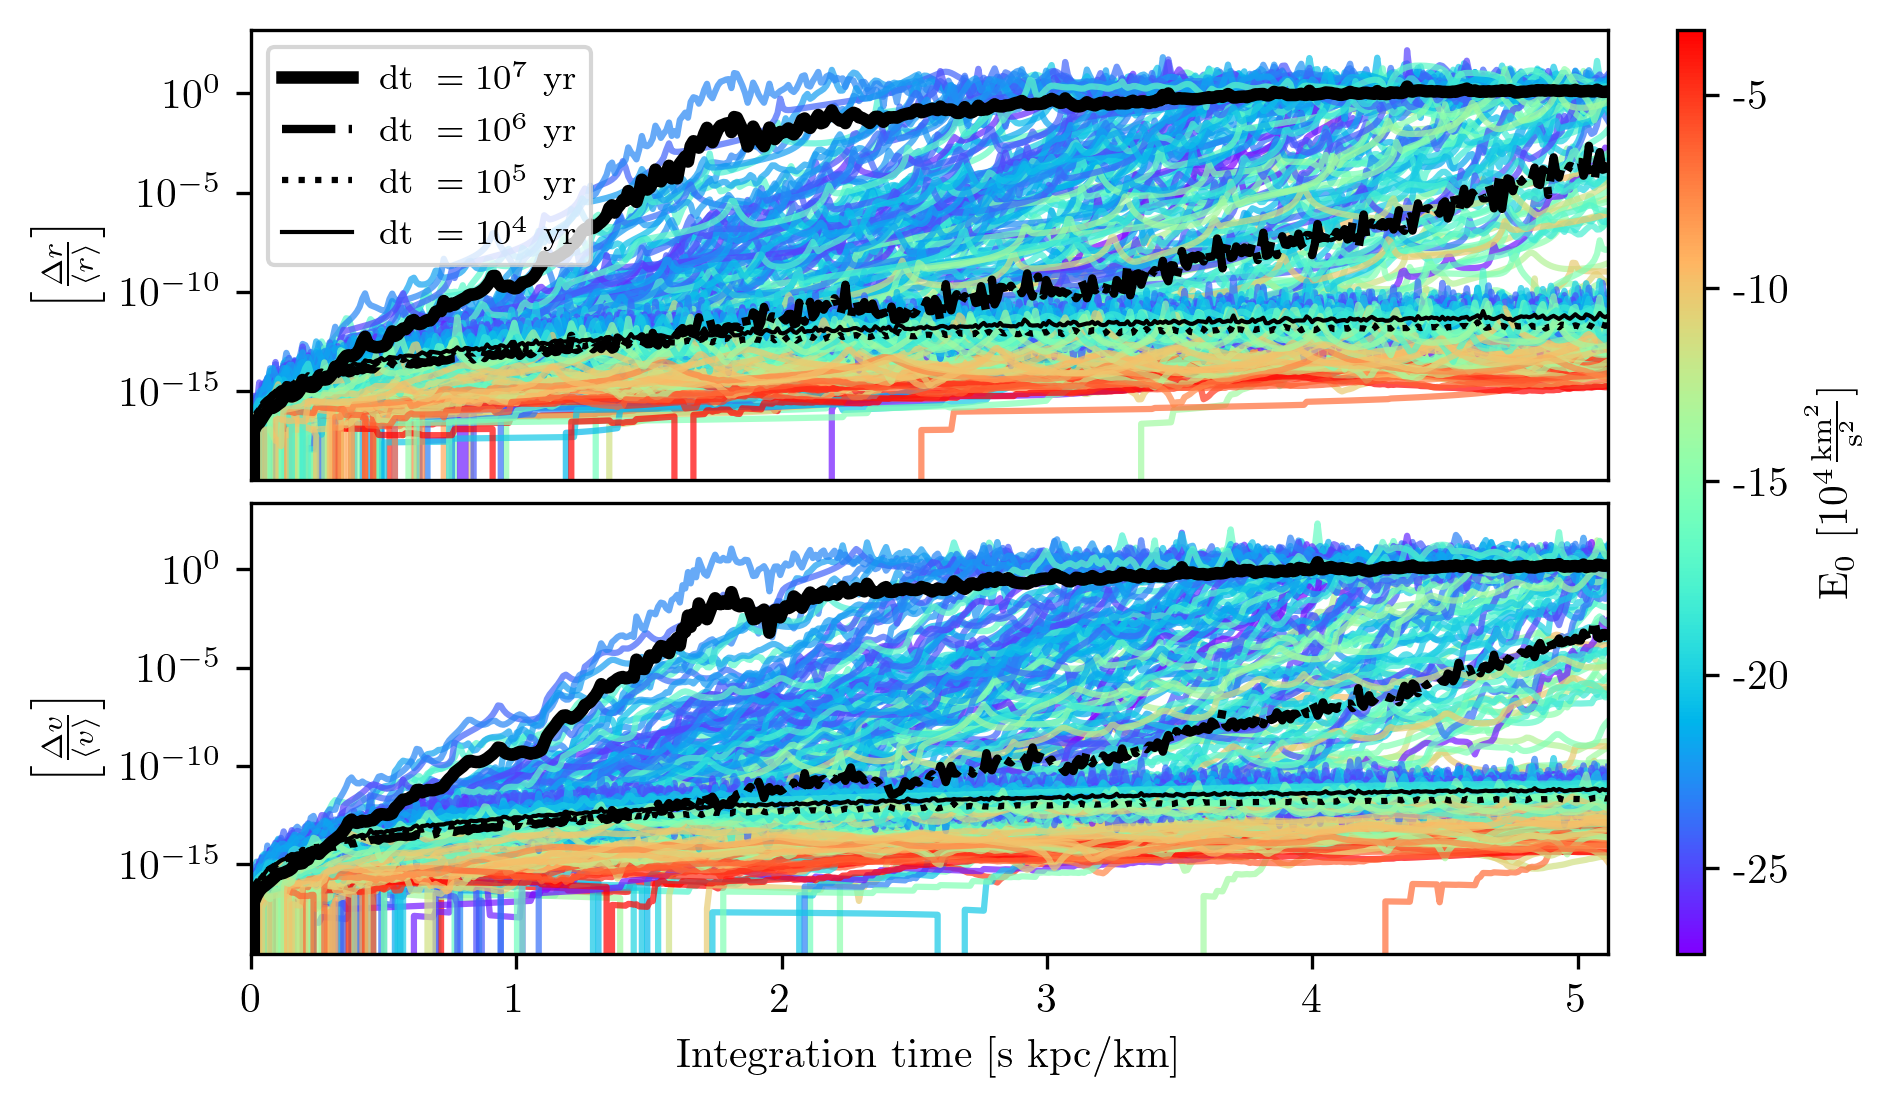
\includegraphics[width=\linewidth]{images/numericalErrorReverseIntegration.png}
            \caption{The \textit{time-reversability} of the Leapfrog scheme for the 165 Galactic globular cluster's for four different time steps indicated in the legend. The whole system is only shown for $10^4$~yr and $10^7$~yr to avoid clutter. The clusters are color-coded to their initial orbital energy just as Fig.~\ref{fig:numericalErrorLeapFrogVanilla}}
            \label{fig:numericalErrorReverseIntegration}
        \end{figure}

        Computation time is quite important. In Fig.~\ref{fig:numericalErrorGlobularClustersComputationTime}, I present the total computation time of integrating the globular cluster system, and the time of a single integration step, which is computed by normalizing the total time by the number of objects and number of steps taken: $T_{\mathrm{total}}/N_{\mathrm{GCs}}/N_{\mathrm{steps}}$. In general, the relationship is linear and the integration time per step per object is roughly constant. The downward trend presented in Fig.~\ref{fig:numericalErrorGlobularClustersComputationTime} is in part a coincidence, as some time realizations minimize this, and in part due to the overhead computation time with initializing and finalizing the calculation contributes less and less with increasing integration time. Nonetheless, for this processor, for a single integration step the mean time is $\sim$ 128~nanoseconds. 
        \begin{figure}
            \centering
            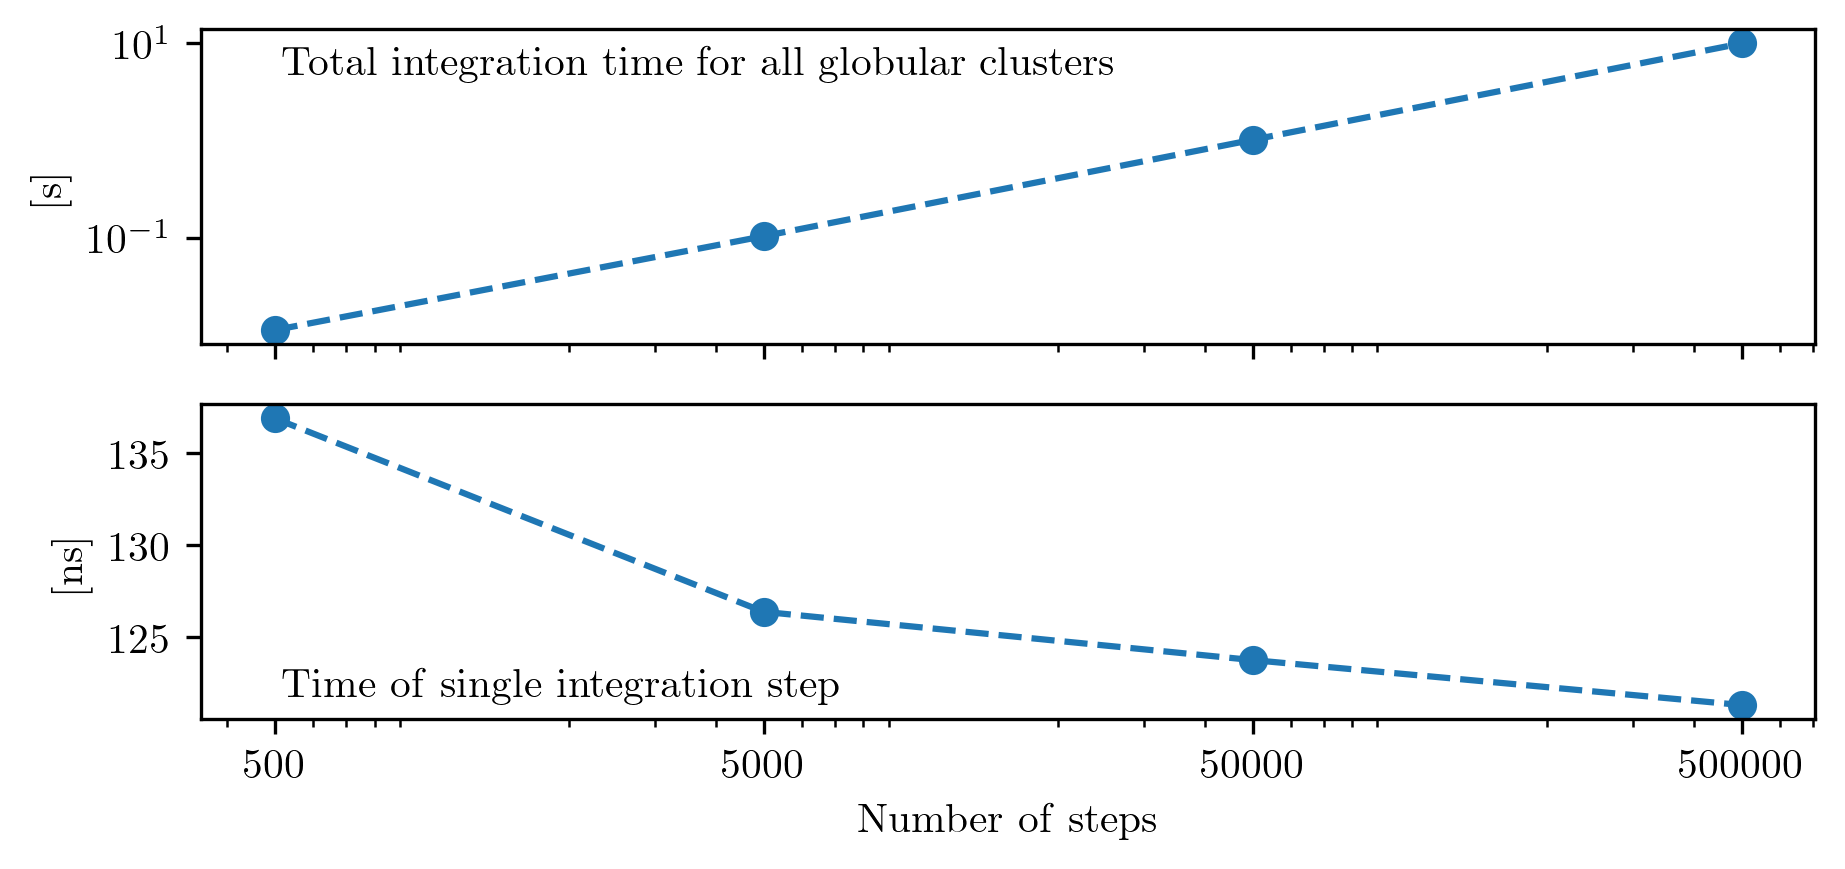
\includegraphics[width=\linewidth]{images/numericalErrorGlobularClustersComputationTime.png}
            \caption{Computation time for integrating the entire globular cluster system using the leapfrog scheme. The top panel shows the total time while the bottom shows computation time for a single step, for a single object being integrated. This was performed on a 2022 MacBook Air with an Apple M2 processor. }
            \label{fig:numericalErrorGlobularClustersComputationTime}
        \end{figure}

        The Ruth-Forest algorithm discussed in the previous section was implemented and is reported in Fig.~\ref{fig:numericalErrorRuthForest}. Here, as expected, we see that the percision greatly increases when decreasing the time step. However, since there are four force evaluations for the for a single timestep, this method is naturally slower perstep than leapfrog. How do the two methods compare over all?
        \begin{figure}
            \centering
            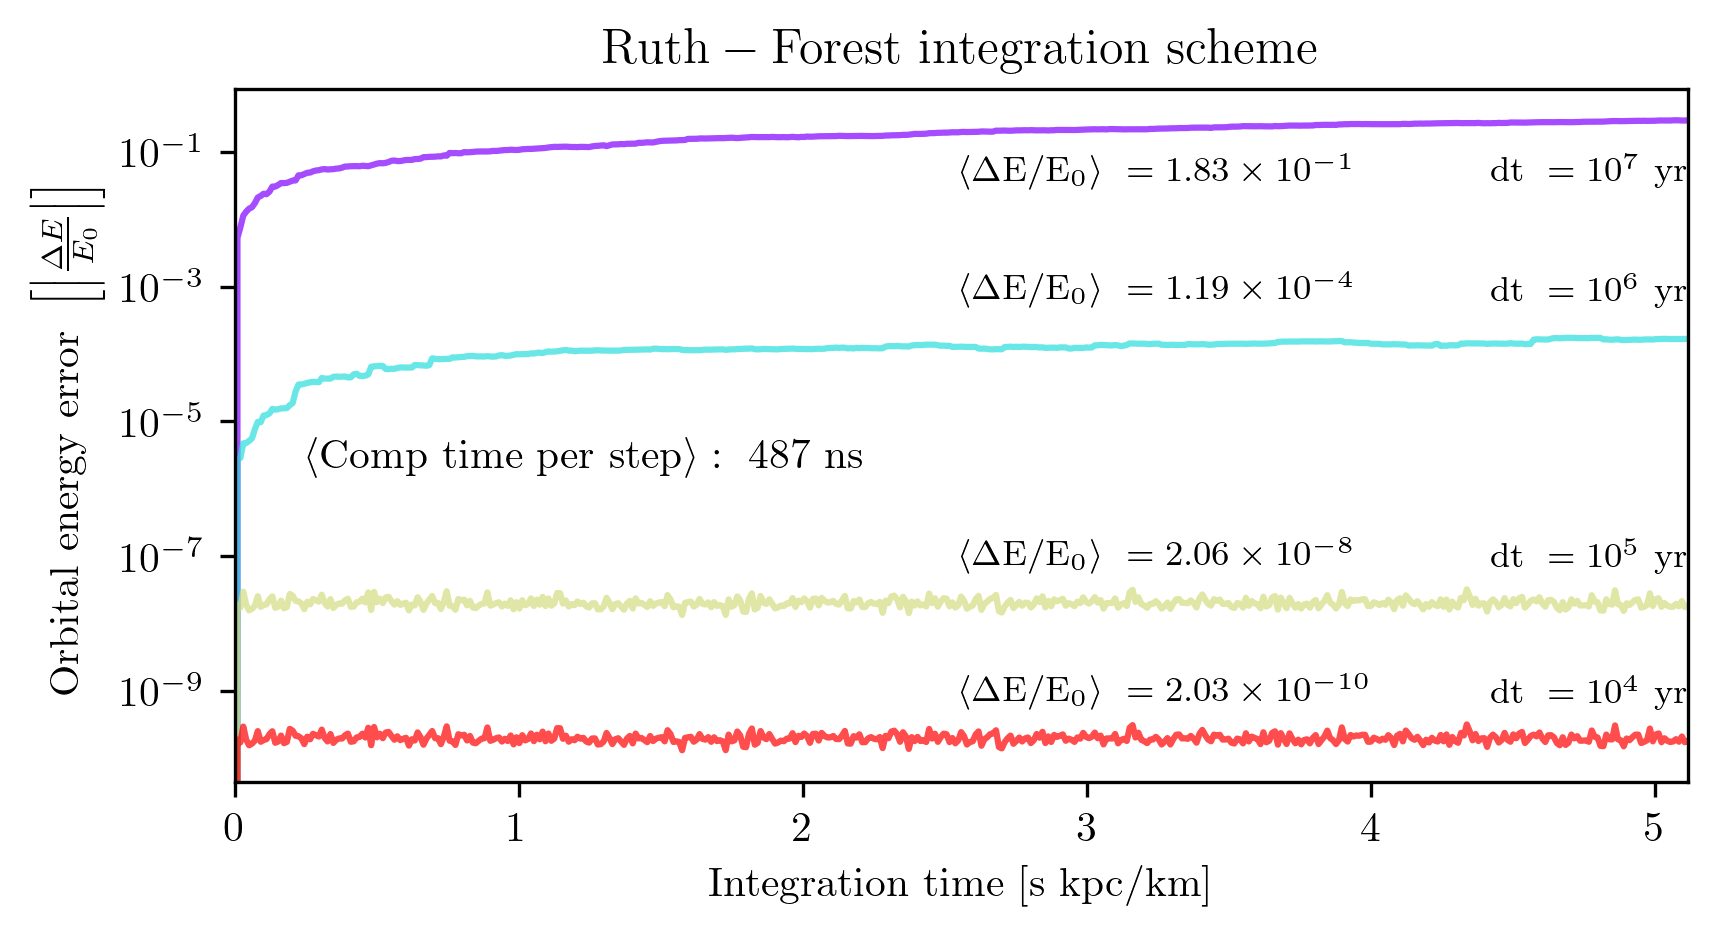
\includegraphics[width=\linewidth]{images/numericalErrorRuthForest.png}
            \caption{The conservation of energy error for the Ruth-Forest integration scheme for the globular cluster system. This plot is similar to Fig.~\ref{fig:numericalErrorLeapFrogVanilla}, but does not preesnt on the whole globular cluster system, just the average error in energy for the whole system with a given time step. The time step and time-average numerical error for the whole system is presented next to each curve. The average computation time per integration step per single object is as well.}
            \label{fig:numericalErrorRuthForest}
        \end{figure}

        In Fig.~\ref{fig:numericalErrorMeanEnergyErrorRuthForestLeapFrog}, I compare the numerical error for again the total number of steps (which is inversely propertial to the time step). It is clear that for a given step size, the Ruth-forest out performs the leap frog, but is it actually better? To answer this question, I fit the two curves with their own trend lines to find the number of steps required to have a relative error of $10^{-8}$. With this requirement, The leapfrog sceme requires 262,641 steps while the Ruth-Forest scheme requires 102,773 steps. However, given the difference in computation time per step, on average, the Forest-Ruth scheme takes $\sim 1.5$x more time for the same degree of numerical precision than the leapfrog. For this reason, I general I use the leapfrog algorithm. In this problem, numerical uncertainties on the order are must less of a limiting factor compared to modeling uncertainties and observational uncertainties, so a better integrator for numerical precision is not worth the pay off of longer computation times. 

        \begin{figure}
            \centering
            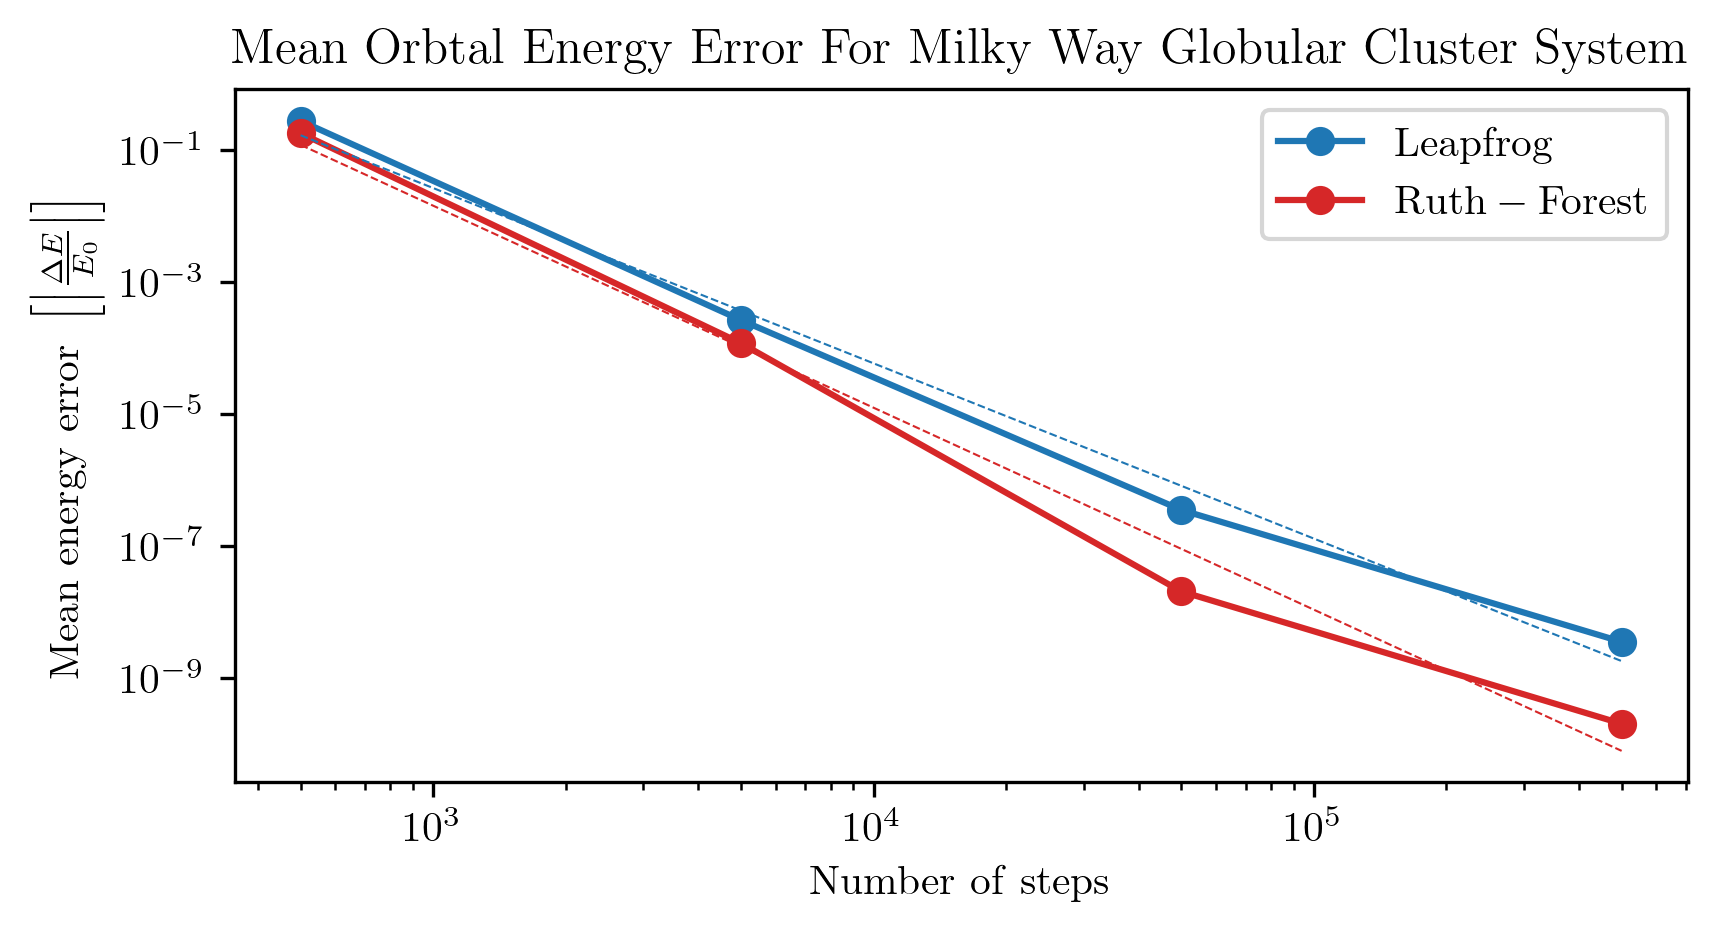
\includegraphics[width=\linewidth]{images/numericalErrorMeanEnergyErrorRuthForestLeapFrog.png}
            \caption{The time averaged error in the conservation of energy for the entire globular cluster system for four different time steps, for two different integration techinques: the Leapfrog against the Ruth-Forest. Their respective trend lines are shown.}
            \label{fig:numericalErrorMeanEnergyErrorRuthForestLeapFrog}
        \end{figure}

    \subsection{Star-particles in a static globular cluster}

        \begin{verbatim}
        VIDEO: cluster_showing_scale_and_dynamical_time.mp4
        \end{verbatim}
        
        A classic problem in astronomy and the physical sciences is that there are two different physical phenomena that are relevent to your problem but they have two very different time scales. This is the case with the globular clusters... Look at Fig.~\ref{fig:GCsystemCharacteristicTimes}. I show a couple different distirbutions.  

        \begin{figure}
            \centering
            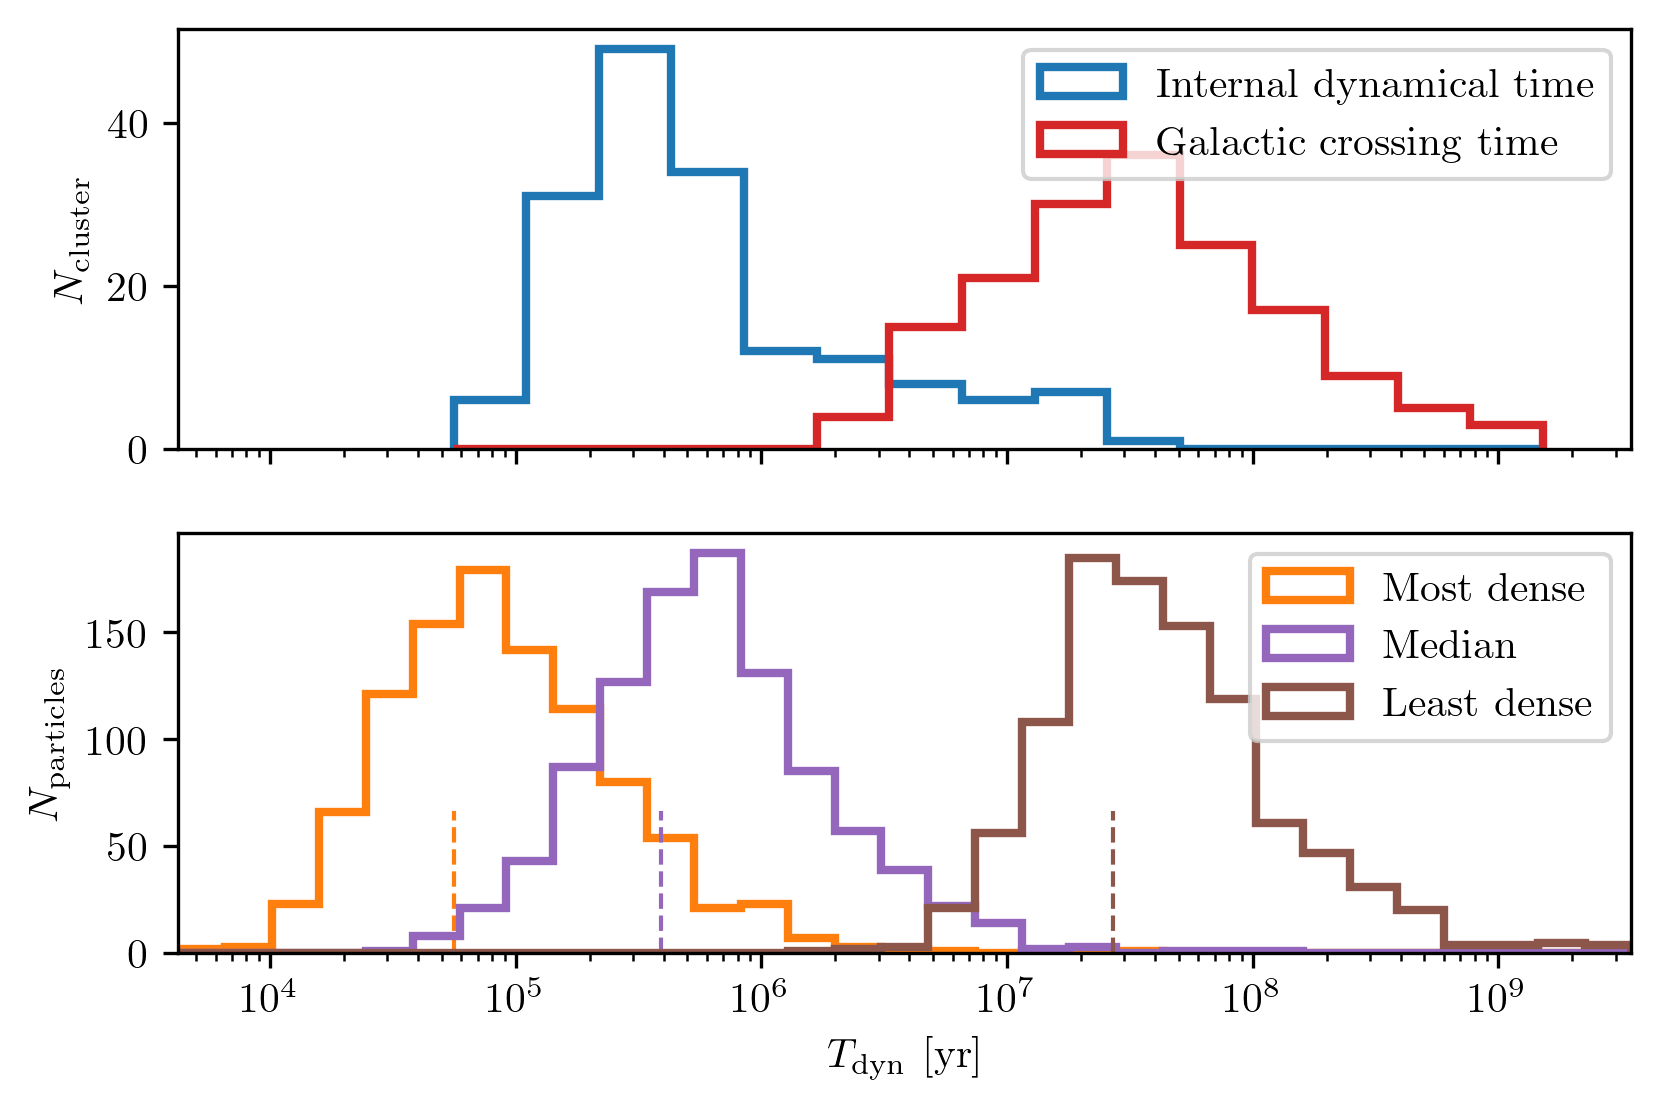
\includegraphics[width=\linewidth]{images/GCsystemCharacteristicTimes.png}
            \caption{The top panel shows orbital characteristic times of the globular cluster system, while the bottom panel shows internal characteristic times for three selected clusters. \textit{Top}: The red distribution shows the orbital crossing time of each cluster within the galaxy, while the blue distribution shows a characteristic internal dynamical time. \textit{Bottom}: The distribution of crossing times for 1,000 sampled star particles within the globular clusters with the smallest, median, and largest internal dynamical times. These times are inversely proportional to the clusters' densities and are computed with isotropic Plummer distributions.}
            \label{fig:GCsystemCharacteristicTimes}
        \end{figure}

        
        \begin{figure}
            \centering
            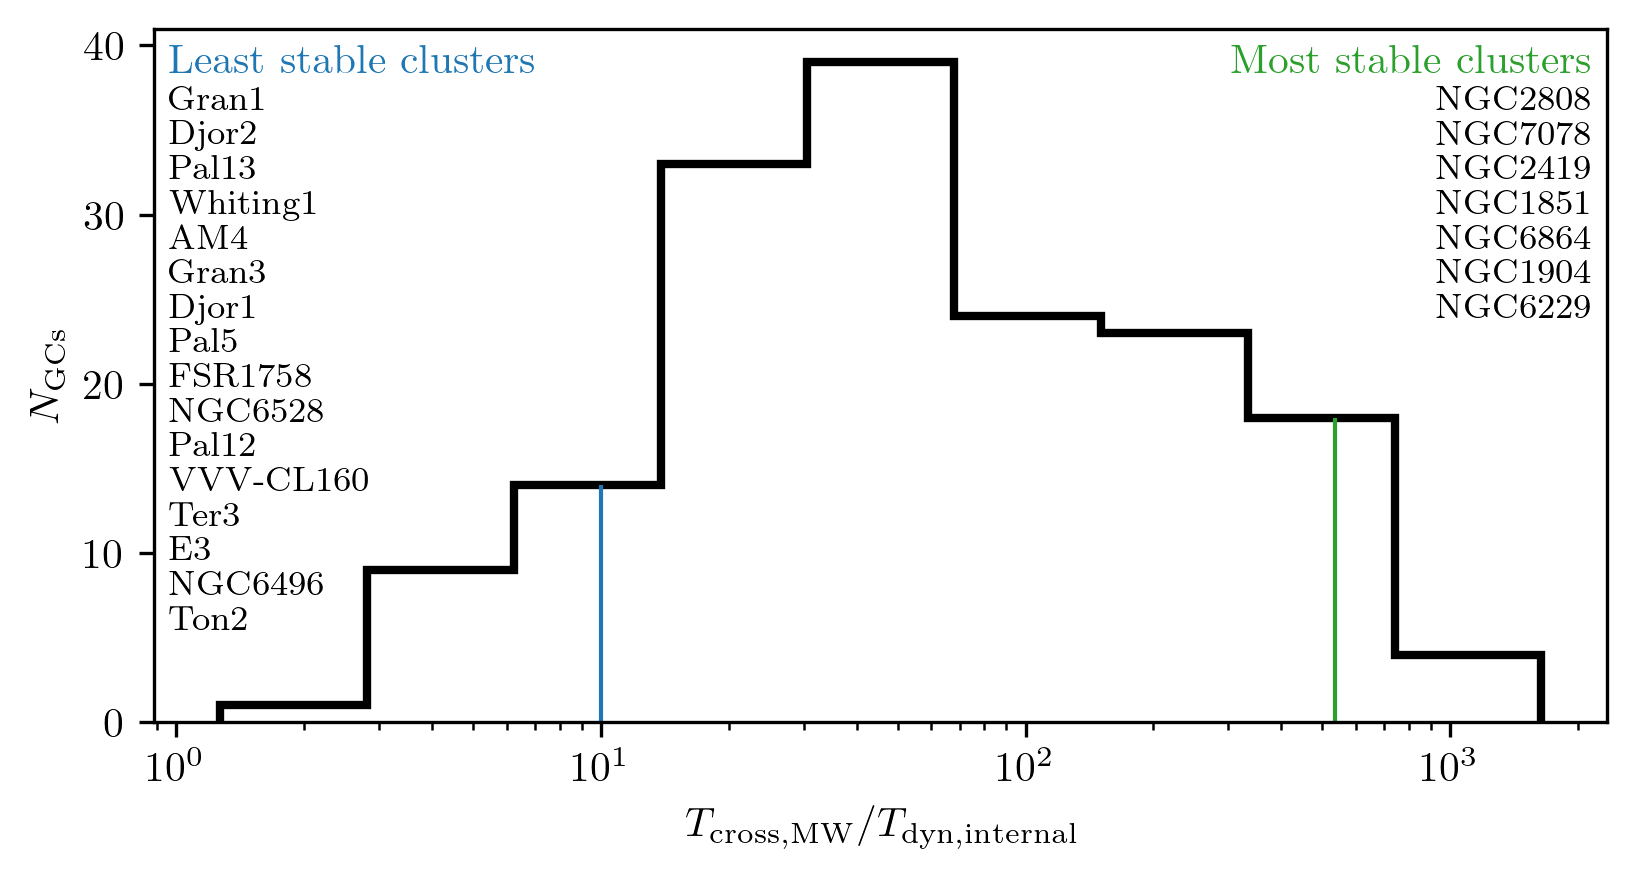
\includegraphics[width=\linewidth]{images/GCsystemStabilityDynamicalTimeRatios.png}
            \caption{Ratio of each globular clusters' galactic crossing time to it's own internal dynamical time, which, individually, are the top distributions from Fig.~\ref{fig:GCsystemCharacteristicTimes}. Clusters' whose dynamical time approaches the crossing time are almost disrupted. Those that are must more dense are far more stable and not close to being disrupted. The vertiable bars show the selected thresholds for each. Both lists present stability in asending order, where Gran~1 is the least stable and NGC~6229 is the most stable. }
        \end{figure}
        How do you choose the number of timesteps? 

        The first is to recognize that

        \begin{equation}
            \Delta t = \frac{T}{N} = \frac{T}{2^{k-1}}
        \end{equation}
        where $N$ is the number of steps and $k$ is the number of intervals. $N$ must be an integer, so our criterion is that ensures the timestep is some fraction of a desired time and one that ensures $N$ properly divides the entire period into $N$-1 equal segments. Our criterion is that the timestep will be some factor $\alpha$ of the dynamical time $\tau_\mathrm{dyn}$. This criterion is thus: 
        \begin{equation}
            \log_2\left(\frac{T}{\alpha \tau_\mathrm{dyn}}\right) + 1 < k.
        \end{equation}
        The smallest number of intervals to make is thus rounding the criterion up to the nearest whole number: $\left\lceil \log_2\left(\frac{T}{\alpha \tau_\mathrm{dyn}}\right) + 1  \right\rceil$. 
        
        
        Now, what is a good $\alpha$ to ensure good conservation of energy and time-reversability? From Fig.~\ref{fig:GCsystemCharacteristicTimes}, we see that the typical globular cluster has a crossing time of $5\times10^{7}~\mathrm{yr}$. From Fig.~\ref{fig:numericalErrorLeapFrogVanilla} that selecting a $\Delta t$ of $10^{4}~\mathrm{yr}$, which is $2\times 10^{-4}$ that of the crossing time, we have conserve energy with a relative error of $10^{-8}$. Then, from Fig.~\ref{fig:numericalErrorReverseIntegration}, we see that $\Delta t= 10^{5}~\mathrm{yr}$ already converges to the best we can do for time-reversability, which is $2\times10^{-3}$ the crossing-time. 


        \begin{figure}
            \centering
            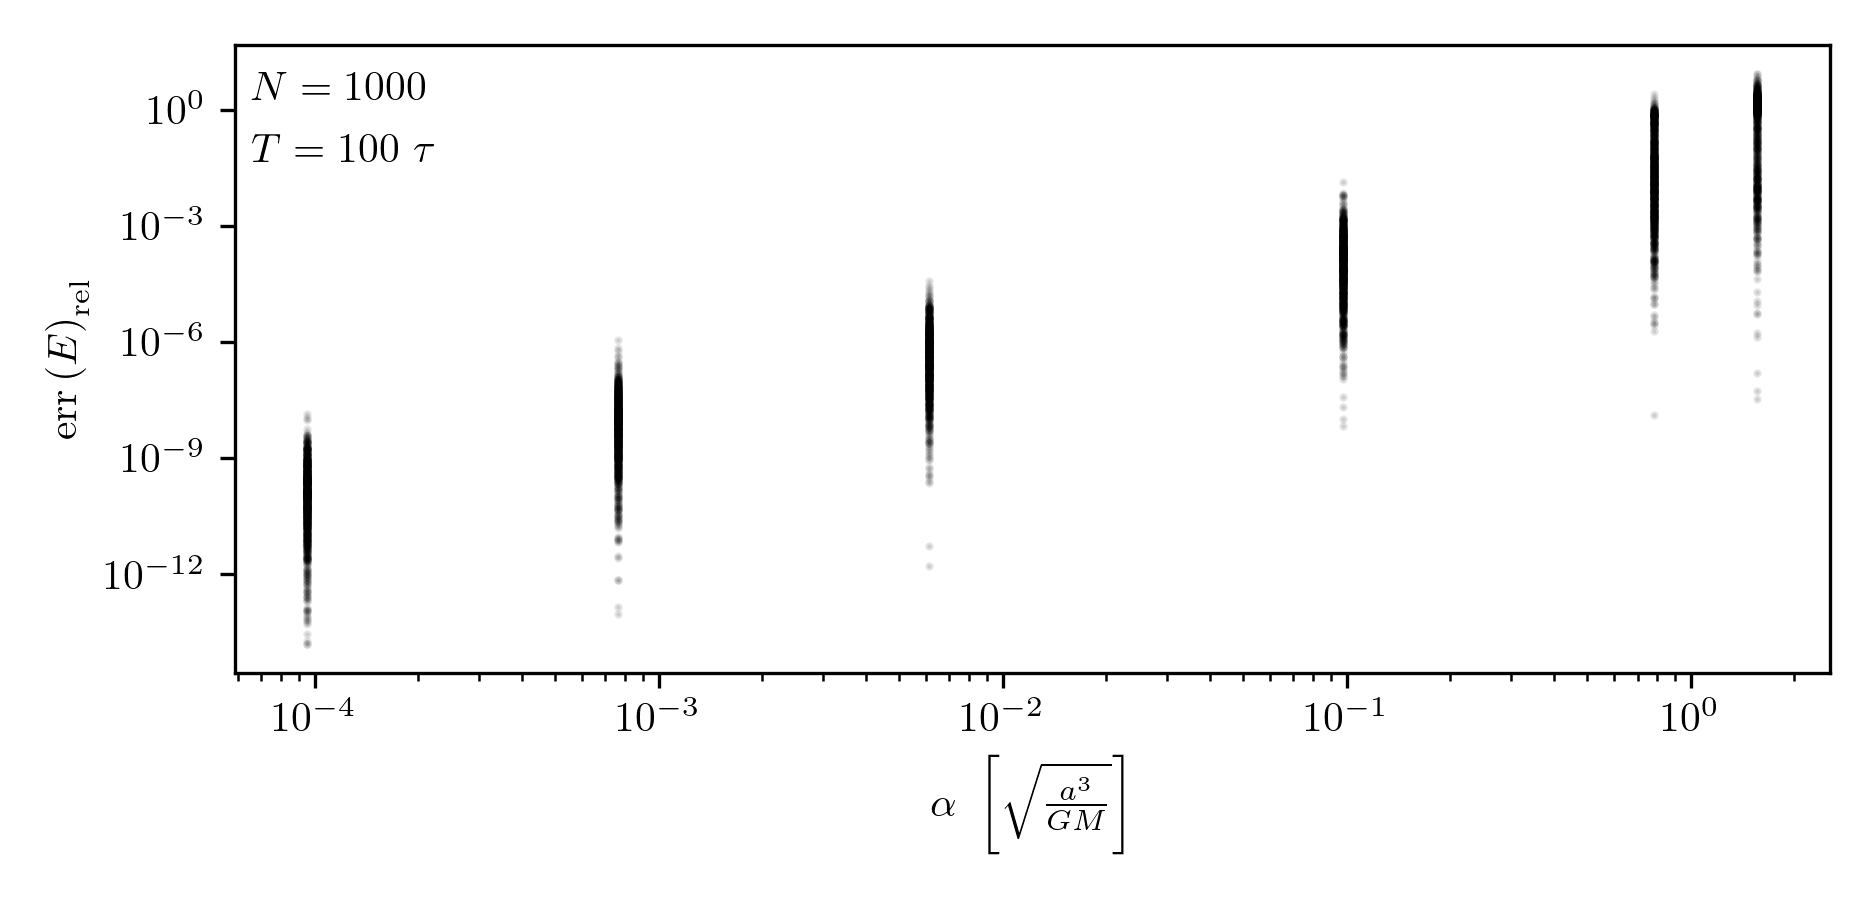
\includegraphics[width=\linewidth]{images/numericalErrorStaticPlummerSphereEnergyError.png}
            \caption{The relative error of the energy conservation for a plummer sphere with different time steps. Each sphere was sampled with a the same number of particles, $N$, and integrated for the same amount of time, $T$, both of which are indicated on the plot. The x-axis is the size of the time-step, $\alpha$, which is the fraction of the internal dynamical time, $\tau = \sqrt{\frac{a^3}{GM}}$. }
            \label{fig:numericalErrorStaticPlummerSphereEnergyError}
        \end{figure}

    \subsection{Full stream generation}

        The preceding sections assessed the numerical stability of integrating globular cluster orbits within the Milky Way, focusing on time-reversibility and relative energy error across two integration schemes: leapfrog and Forest-Ruth. I also considered the computational cost associated with different temporal resolutions. Separately, I evaluated the energy conservation for star particles evolving within a stationary Plummer sphere, quantifying the relative error as a function of timestep. In that context, the cluster's potential was scaled to its scale radius, mass, and the gravitational constant. This non-dimensionalization allowed me to select timesteps as fractions of the internal dynamical time $\tau$ of each cluster. 


        In this section, I combine these two components: I examine the quality of orbit integration for star particles evolving within a globular cluster, itself orbiting in the Galactic potential.


        I restrict the analysis here to the leapfrog integrator for two main reasons. First, although the Forest-Ruth scheme achieves better energy conservation (see Fig.~\ref{fig:numericalErrorMeanEnergyErrorRuthForestLeapFrog}), this comes at a significantly higher computational cost, which outweighs its marginal gains for this application. Second, the equations of motion used to model stream generation (see Eq.~XXX in the theory chapter) require loading the center-of-mass orbit of the host cluster at each simulation time. Because Forest-Ruth evaluates forces at non-uniform substeps, using it would require either: (1) storing and loading the cluster orbit at each substep, which would demand excessive disk space and complex code restructuring; or (2) interpolating the orbit at intermediate times, which introduces ambiguity regarding whether time-reversibility is preserved with linear or cubic interpolation. For these reasons, I opted not to explore Fores-Ruth further in the context of full stream generation.

        To assess the performance of the stream-generation method, I designed a quality assurance experiment illustrated in Fig.~\ref{fig:NumericalErrorStreamRetrace_NGC6171_Nsteps_524288_stepsPerTau_155}. I began by integrating the orbit of a globular cluster's center of mass backward in time by 1 Gyr. At this point, a Plummer sphere was sampled using the cluster's half-mass radius and mass, with 512 star particles. This system was translated to the center-of-mass phase-space coordinates and then integrated forward in time to the present day, forming a stream. I saved the resulting positions and computation time. To assess time-reversibility, I then integrated the stream particles backward again for 1 Gyr.

        A note on terminology: although the cluster orbit is initialized from present-day observations, in the context of stream generation, I refer to the past position (1 Gyr ago) as the ``initial conditions''. The forward-integrated system represents the ``stream'', and the backward-integrated version of the stream is referred to as the ``retrace''.

        Figures~\ref{fig:NumericalErrorStreamRetrace_NGC6171_Nsteps_524288_stepsPerTau_155} and \ref{fig:NumericalErrorStreamRetrace_NGC6171_Nsteps_4096_stepsPerTau_1} show the results of this experiment across four different timesteps. As expected, increasing the timestep degrades time-reversibility and worsens energy conservation.

        \begin{figure}
            \centering
            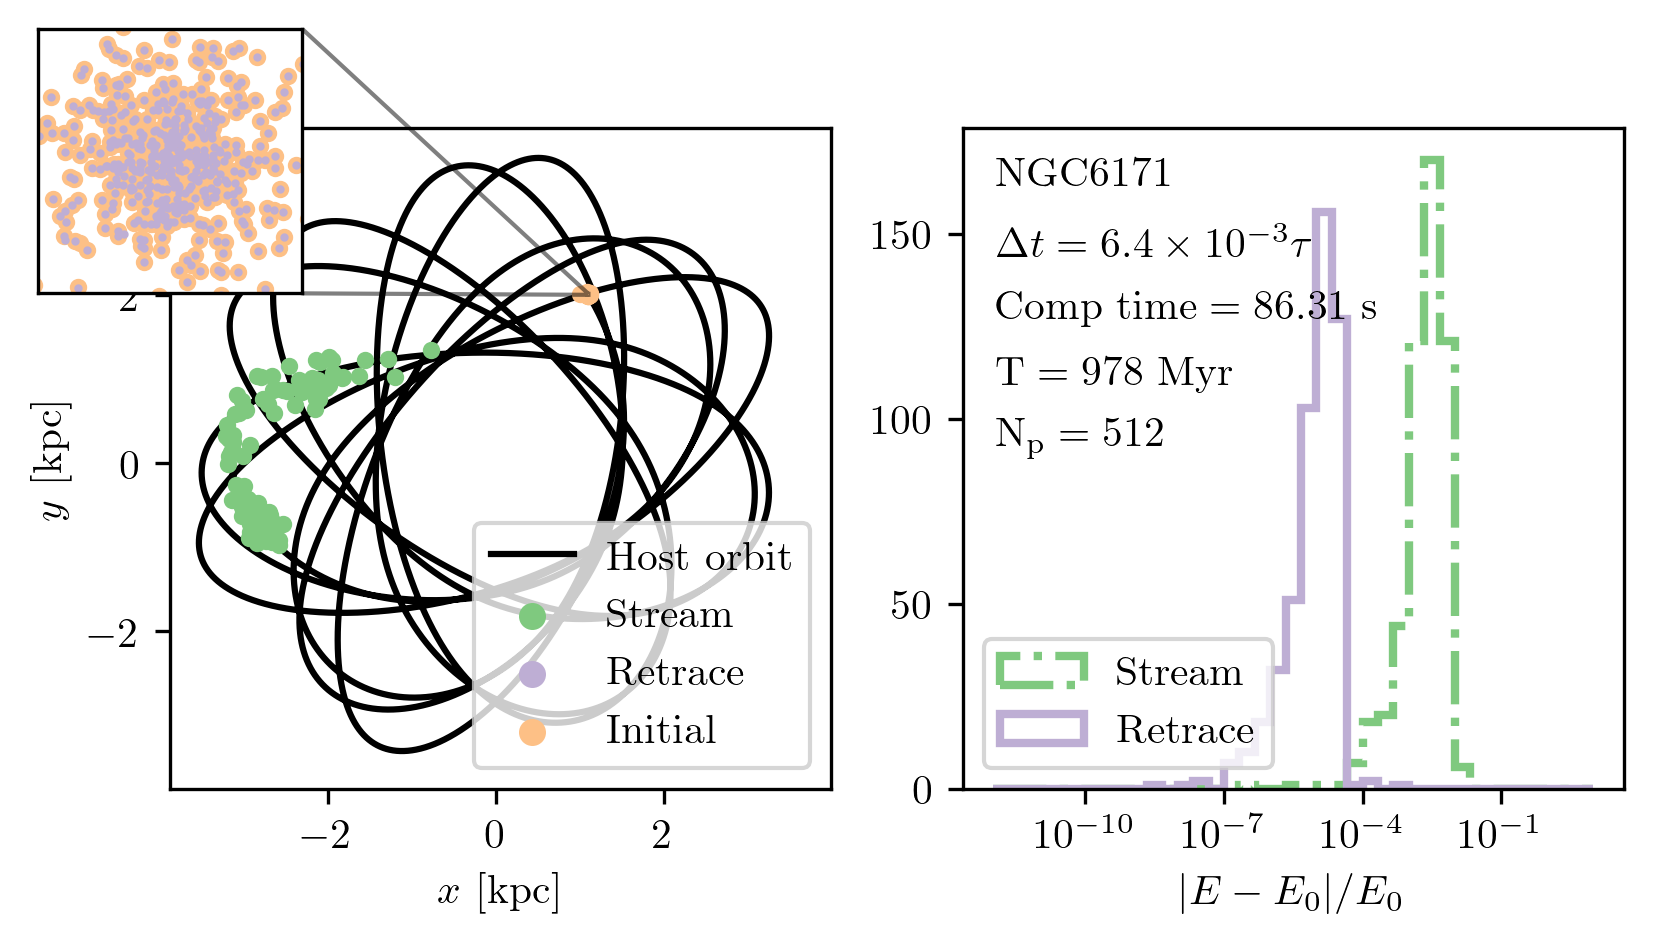
\includegraphics[width=\linewidth]{images/NumericalErrorStreamRetrace_NGC6171_Nsteps_524288_stepsPerTau_155.png}
            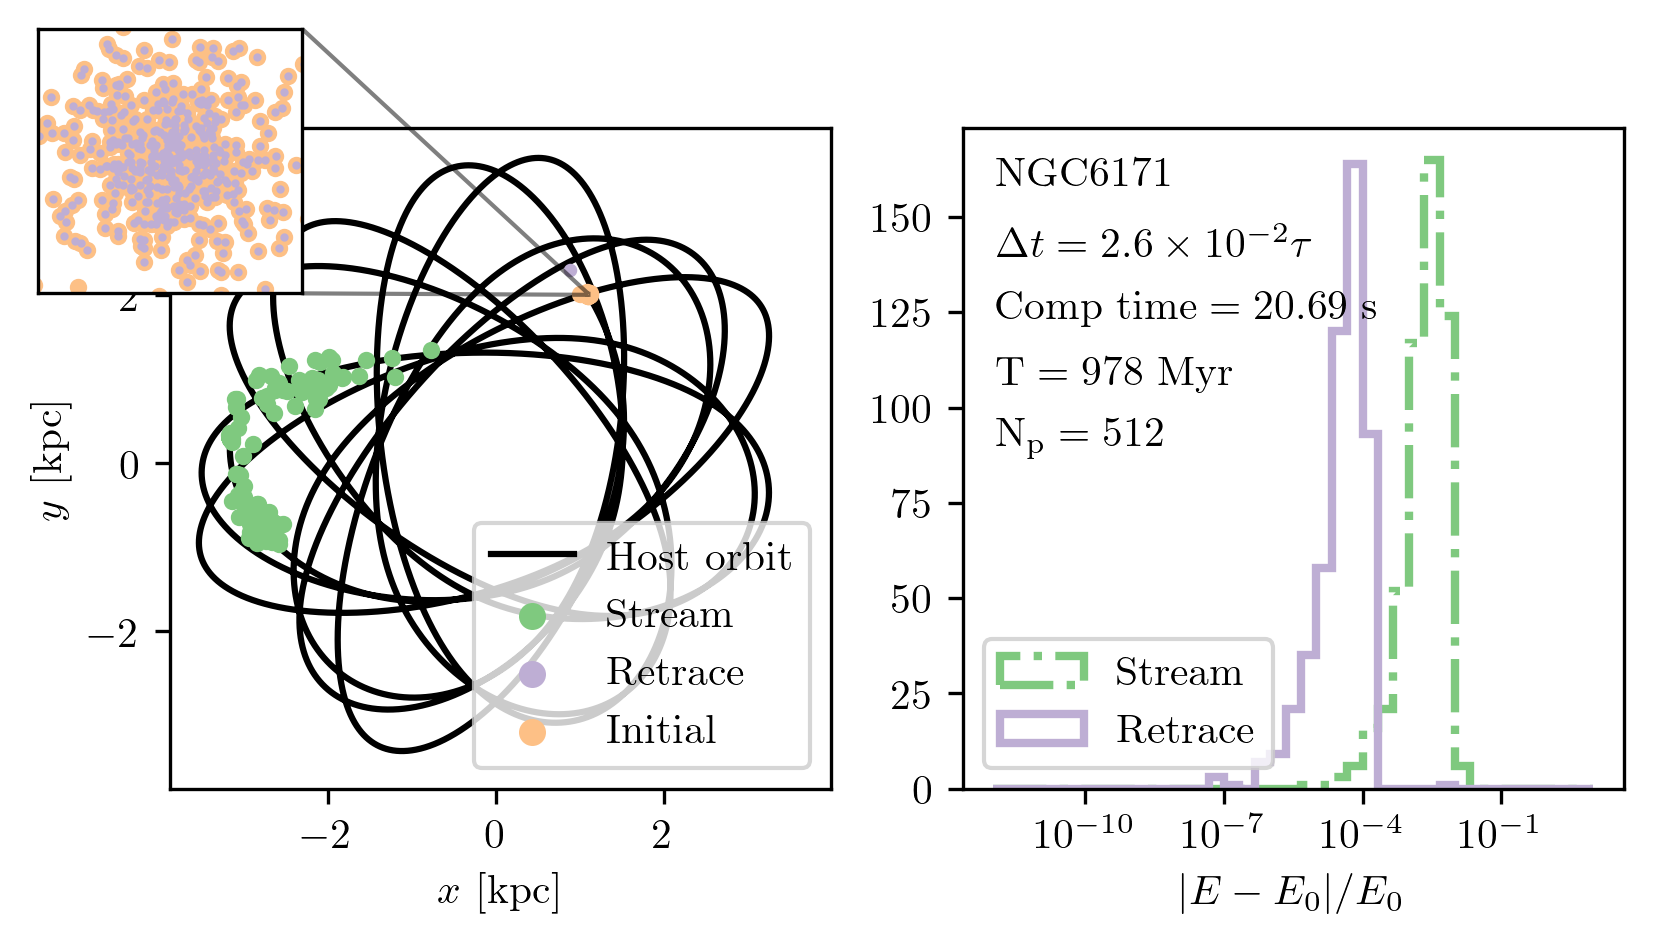
\includegraphics[width=\linewidth]{images/NumericalErrorStreamRetrace_NGC6171_Nsteps_131072_stepsPerTau_38.png}
            \caption{Time-reversibility test for NGC~6171. The cluster's orbit was integrated backward by 1 Gyr, and a Plummer sphere of 512 particles was initialized at that position ("Initial"). The system was then integrated forward ("Stream") and backward again ("Retrace"). Right panels show the relative error in energy. The timestep was selected as a fraction of the internal dynamical time $\tau$.}
            \label{fig:NumericalErrorStreamRetrace_NGC6171_Nsteps_524288_stepsPerTau_155}
        \end{figure}


        \begin{figure}
            \centering
            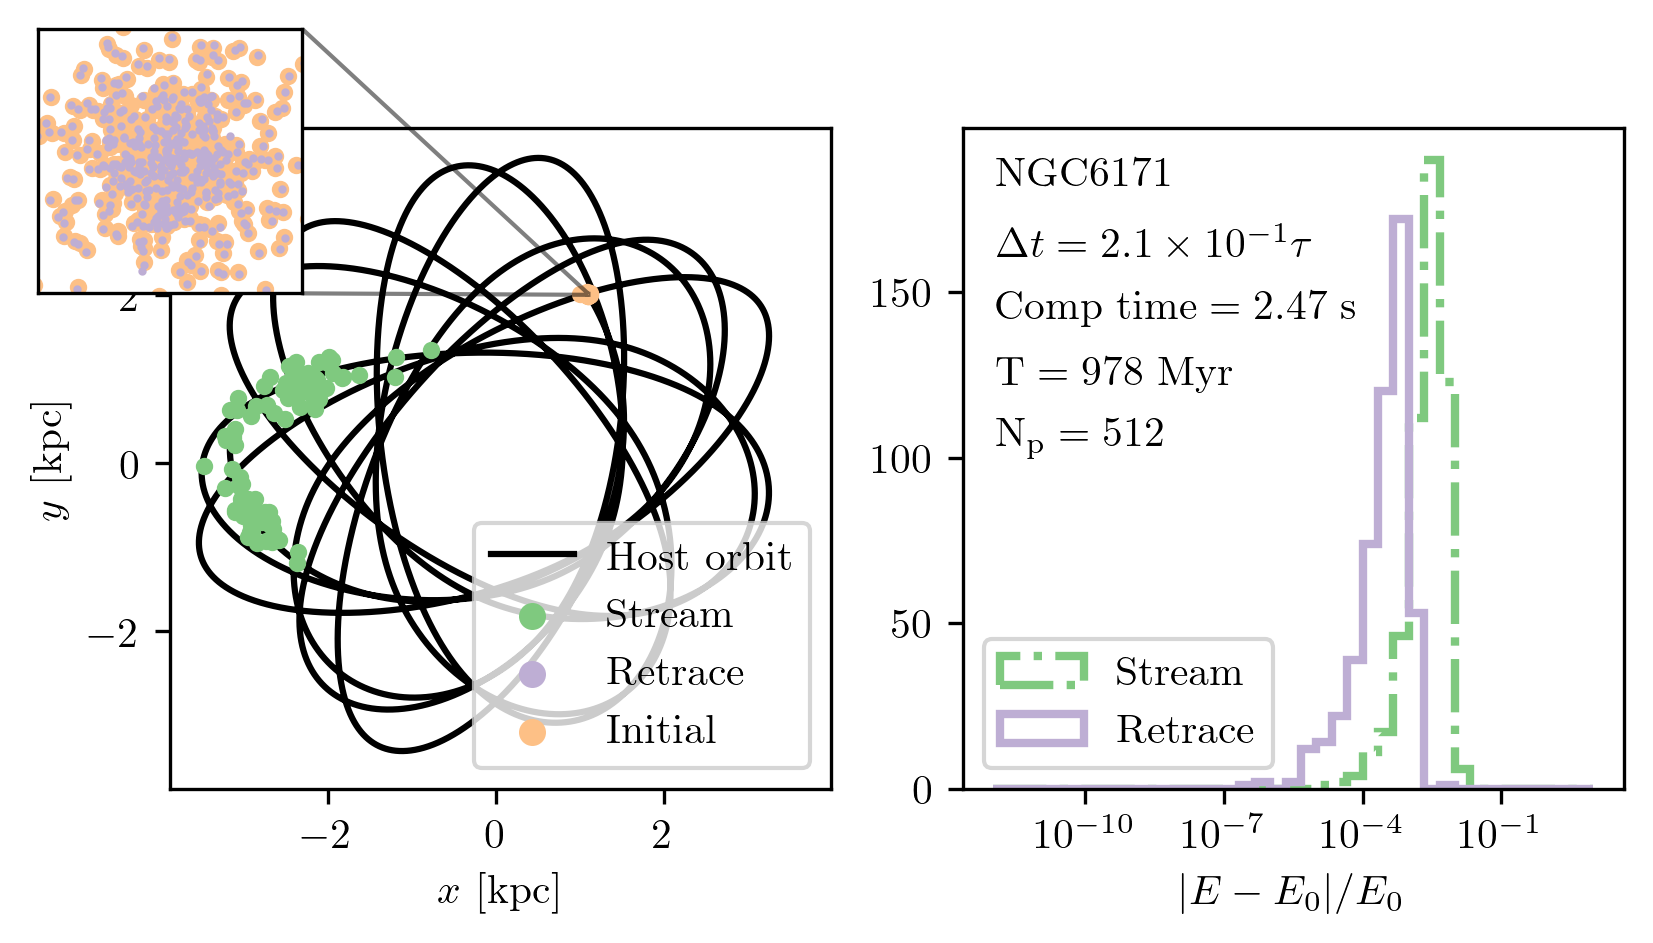
\includegraphics[width=\linewidth]{images/NumericalErrorStreamRetrace_NGC6171_Nsteps_16384_stepsPerTau_4.png}
            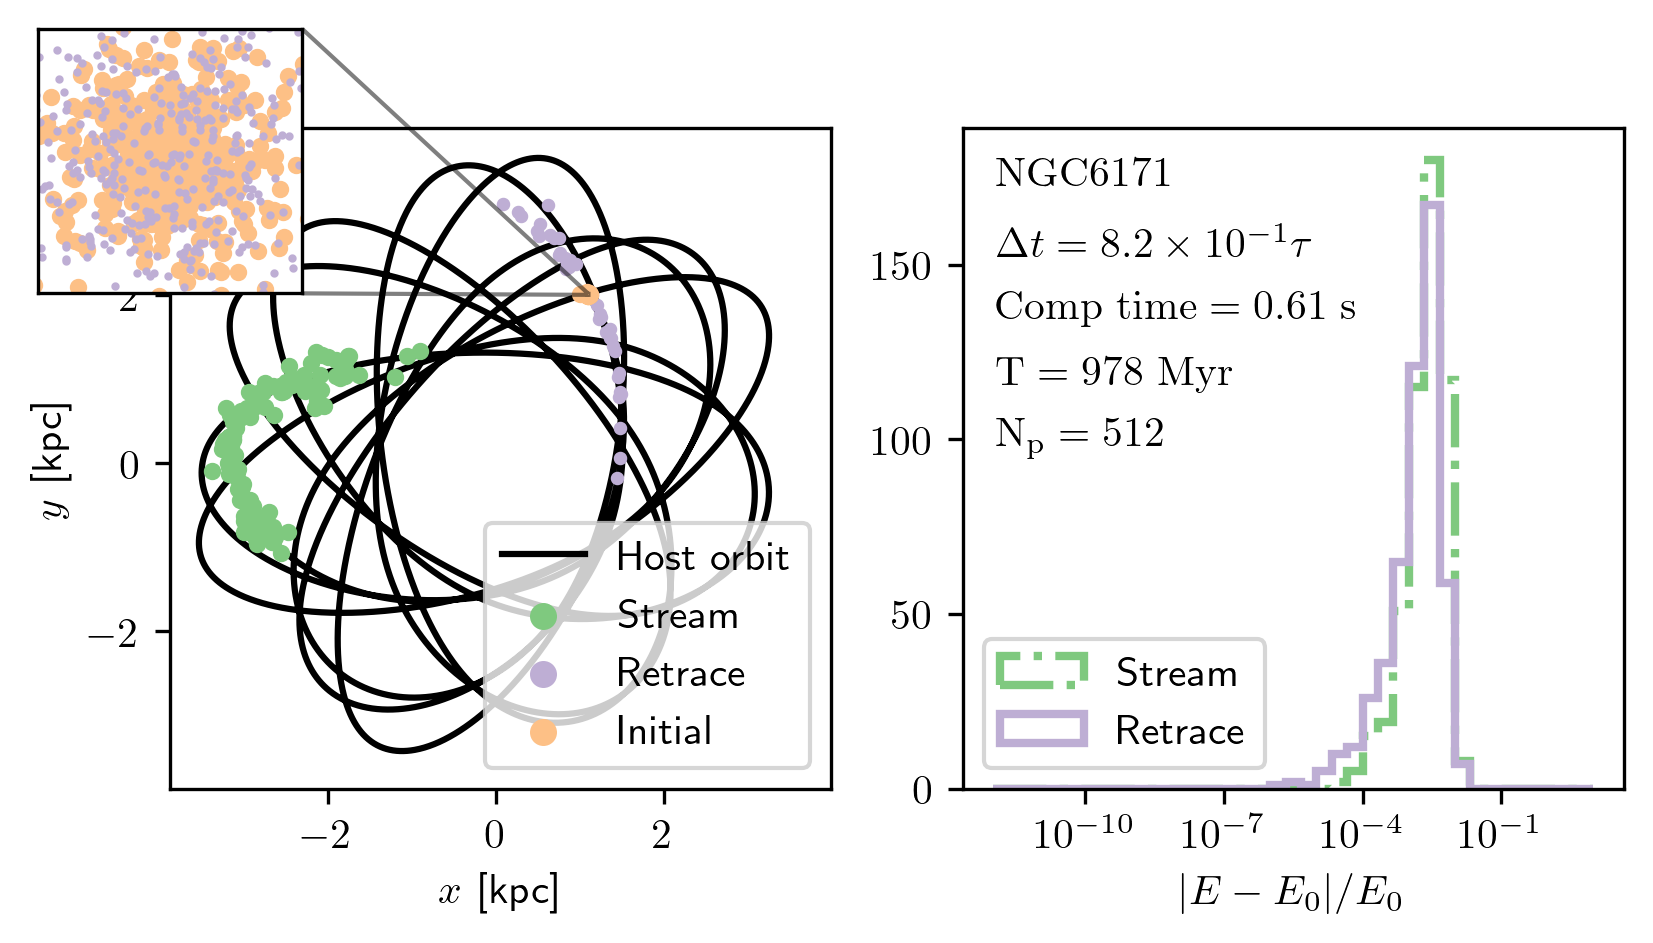
\includegraphics[width=\linewidth]{images/NumericalErrorStreamRetrace_NGC6171_Nsteps_4096_stepsPerTau_1.png}
            \caption{Same experiment as in Fig.~\ref{fig:NumericalErrorStreamRetrace_NGC6171_Nsteps_524288_stepsPerTau_155}, but using larger timesteps as indicated. Time-reversibility and energy conservation degrade as timestep increases.}
            \label{fig:NumericalErrorStreamRetrace_NGC6171_Nsteps_4096_stepsPerTau_1}
        \end{figure}

        The two smaller timesteps in Fig.~\ref{fig:NumericalErrorStreamRetrace_NGC6171_Nsteps_524288_stepsPerTau_155} sufficiently retrace the cluster's initial configuration. I compare each particle's energy change between its initial and retraced state. For $\Delta t \sim 6\times10^{-3}~\tau$, the relative energy errors in the retraced state fall mostly between $10^{-7}$ and $10^{-4}$. For $\Delta t \sim 3\times10^{-2}~\tau$, the distribution shifts upward by about an order of magnitude, indicating reduced accuracy.

        Interestingly, the energy distributions at the present-day timestep (i.e., for the stream) fall between $10^{-4}$ and $10^{-1}$ across all cases, and are largely insensitive to timestep. This is expected: the equations of motion are time-dependent due to the non-autonomous external Galactic potential, so energy is not conserved by design. The fact that energy errors do not vary strongly with timestep suggests that even the coarsest resolutions used here are adequate for capturing the global motion within the Galactic potential. As shown in Figs.~\ref{fig:numericalErrorLeapFrogVanilla} and \ref{fig:numericalErrorRuthForest}, timesteps of $\sim10^5$ years are sufficient for stable orbit integration. Even the largest timestep used in the bottom panel of Fig.~\ref{fig:NumericalErrorStreamRetrace_NGC6171_Nsteps_4096_stepsPerTau_1} corresponds to $\sim10^5$ years—comparable to the cluster's internal dynamical time.

        Although energy is not conserved in these simulations—since the Hamiltonian includes a time-dependent Galactic potential—we find that the energy change for stream particles remains bounded around a relative error of $10^{-1}$. Why is this the case?

        Consider a thought experiment: suppose the globular cluster were removed, and the stars were left to orbit freely in the Galactic potential. The initial velocities and positions of the stars would still reflect the distribution sampled from the Plummer sphere. As a result, they would exhibit a range of orbital energies rather than a single value. This intrinsic energy spread, denoted $\sigma_E$, is not a numerical artifact but a physical property of the system's initial conditions.

        The relative spread in energies, $\sigma_E / E_0$, where $E_0$ is the mean orbital energy of the system, provides an estimate of the apparent "energy error" we observe. We can make a rough estimate of this ratio by comparing the internal potential energy scale of the cluster to its orbital energy in the Galaxy. The characteristic internal potential is on the order of $\Phi \sim GM/a$, where $M \sim 10^5~M_\odot$ and $a \sim 0.005$~kpc, yielding $\Phi \sim 10^2~\mathrm{km}^2\,\mathrm{s}^{-2}$. In contrast, the typical orbital energy of a globular cluster in the Milky Way is about $10^5~\mathrm{km}^2\,\mathrm{s}^{-2}$ (see Fig.~\ref{fig:energy_sensitivity_analysis_MWGCS_to_distance_RV_mu}). 

        This discrepancy of roughly three orders of magnitude implies that the intrinsic energy spread from the initial Plummer sampling is about $10^{-3}$ times the absolute orbital energy. However, since we are examining the energy relative to each particle's initial value—which is small—the observed fractional differences cluster around $\sim 10^{-1}$, consistent with what we measure in the stream. Thus, the apparent energy ``error'' reflects not integration drift but the physical energy distribution inherited from the initial conditions.

        Fig.~\ref{fig:NumericalErrorStreamRetrace_NGC6171_Nsteps_524288_stepsPerTau_155} \& Fig.~\ref{fig:NumericalErrorStreamRetrace_NGC6171_Nsteps_4096_stepsPerTau_1} demonstrate the case of a single cluster. How is the energy conservation for the entire catalog? In Fig.~\ref{fig:NumericalErrorStreamRetraceEnergyConservation} I present the realtive error in the conservation of energy for retracing the orbit of each individual star particle per globular cluster for each cluster in the catalog. Each data point reports the mean error in the conservation of energy. Each cluster was integrated for 5~Gyr. The upper limits for the timesteps were sampeld logarithmically between $10^{0}$ and $10^{-2}$. 

        From inspecting Fig.~\ref{fig:NumericalErrorStreamRetrace_NGC6171_Nsteps_524288_stepsPerTau_155}, a time step less than $3\times10^{-2}~\tau$ is great for retracing the orbit of each star particle and even $2\times10^{-1}~\tau$ isn't horrible. This would place the retrace energy conservation between $10^{-5}-10^{-3}$ on average per system. 

        \begin{figure}
            \centering 
            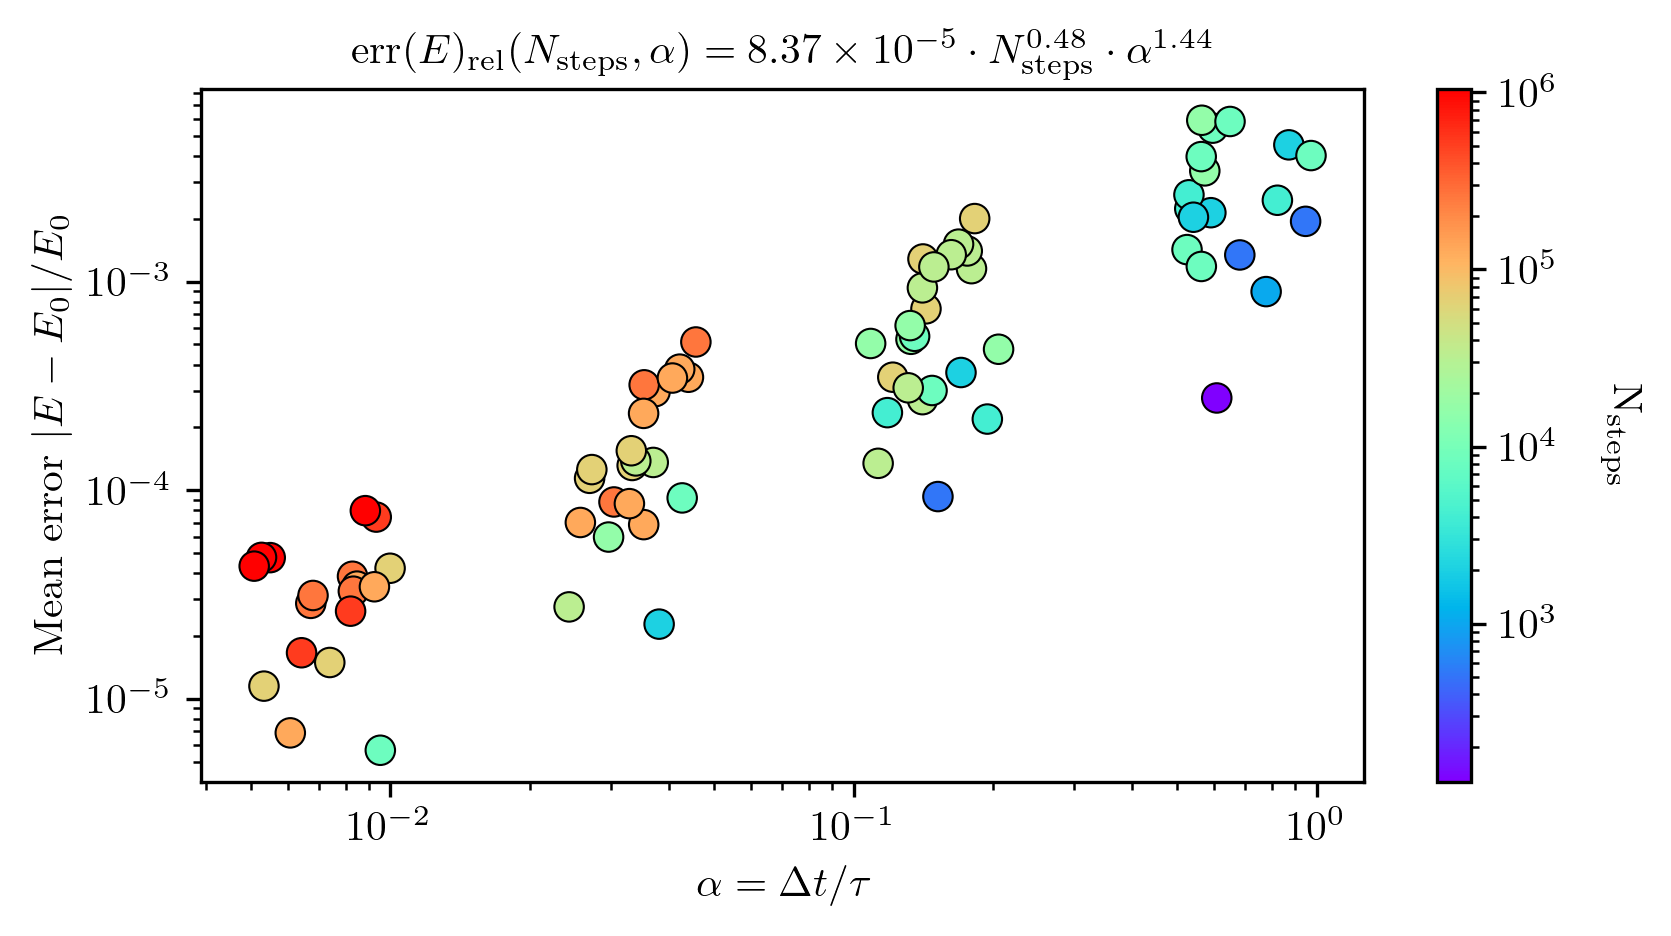
\includegraphics[width=\linewidth]{images/NumericalErrorStreamRetraceEnergyConservation.png}
            \caption{The conservation of energy for the retrace of each globular cluster in the catalog. Each cluster was sampled with 512 particles and integrated for 5~Gyr. Four upper thresholds for each time step were logarithmically sampled between $10^{0}$ and $10^{-2}$, and selected individually for each cluster in combination with it's internal dynamical time that evenly divided the integration time. }
            \label{fig:NumericalErrorStreamRetraceEnergyConservation}
        \end{figure}

        The quality of the solutions is fundamental for proper results. However, computation time and cost is also very important. The spirit of choosing to solve the restricted three body problem instead of modeling the system as an N~body for a faster computation. With N~body, the computation time should scale with $N_p^2$, while for the restricted three body problem it should scale with $N_p$. For both, it should scale linearly with the number of integration steps. 

        How does $tstrippy$ perform? In Fig.~\ref{fig:NumericalErrorComputationTimeScalingForStreams}, I launched an experiment with all the globular clusters integrating them each for 1~Gyr. I choose the timestep to be at most 1/20 of each internal dynamical time, thus since each cluster has a different dynamical time, it will require a different number of steps. For each of these tests I use $10^1,~10^2,~10^2,~10^3$ particles and launched them on cluster at the paris observatory. Then, I fit a scaling law of $C(N_p,N_s) = \langle C\rangle N_p^a N_s^b$. If the code scales linearly, then each exponent, $a,~b$, should be 1 and $\langle C\rangle$ would be the mean computation time. 
        
        Fig~\ref{fig:NumericalErrorComputationTimeScalingForStreams} shows that the code is \textit{less} efficient than linear scaling with number of particles, since the best fit exponent is $1.35$. However, it scales \textit{better} than linear with the number of steps. Perhaps this can be explained by the fact that there is overhead time involved for initiating and ending each simulation. Is there are more steps, this overhead time gets proportionally smaller. Since the power law has an exponent of $0.95$, the overhead is marginal. However, it is excellent that the exponent is not greater than 1, which would mean the code would slow down with execution time. 


        \begin{figure}
            \centering
            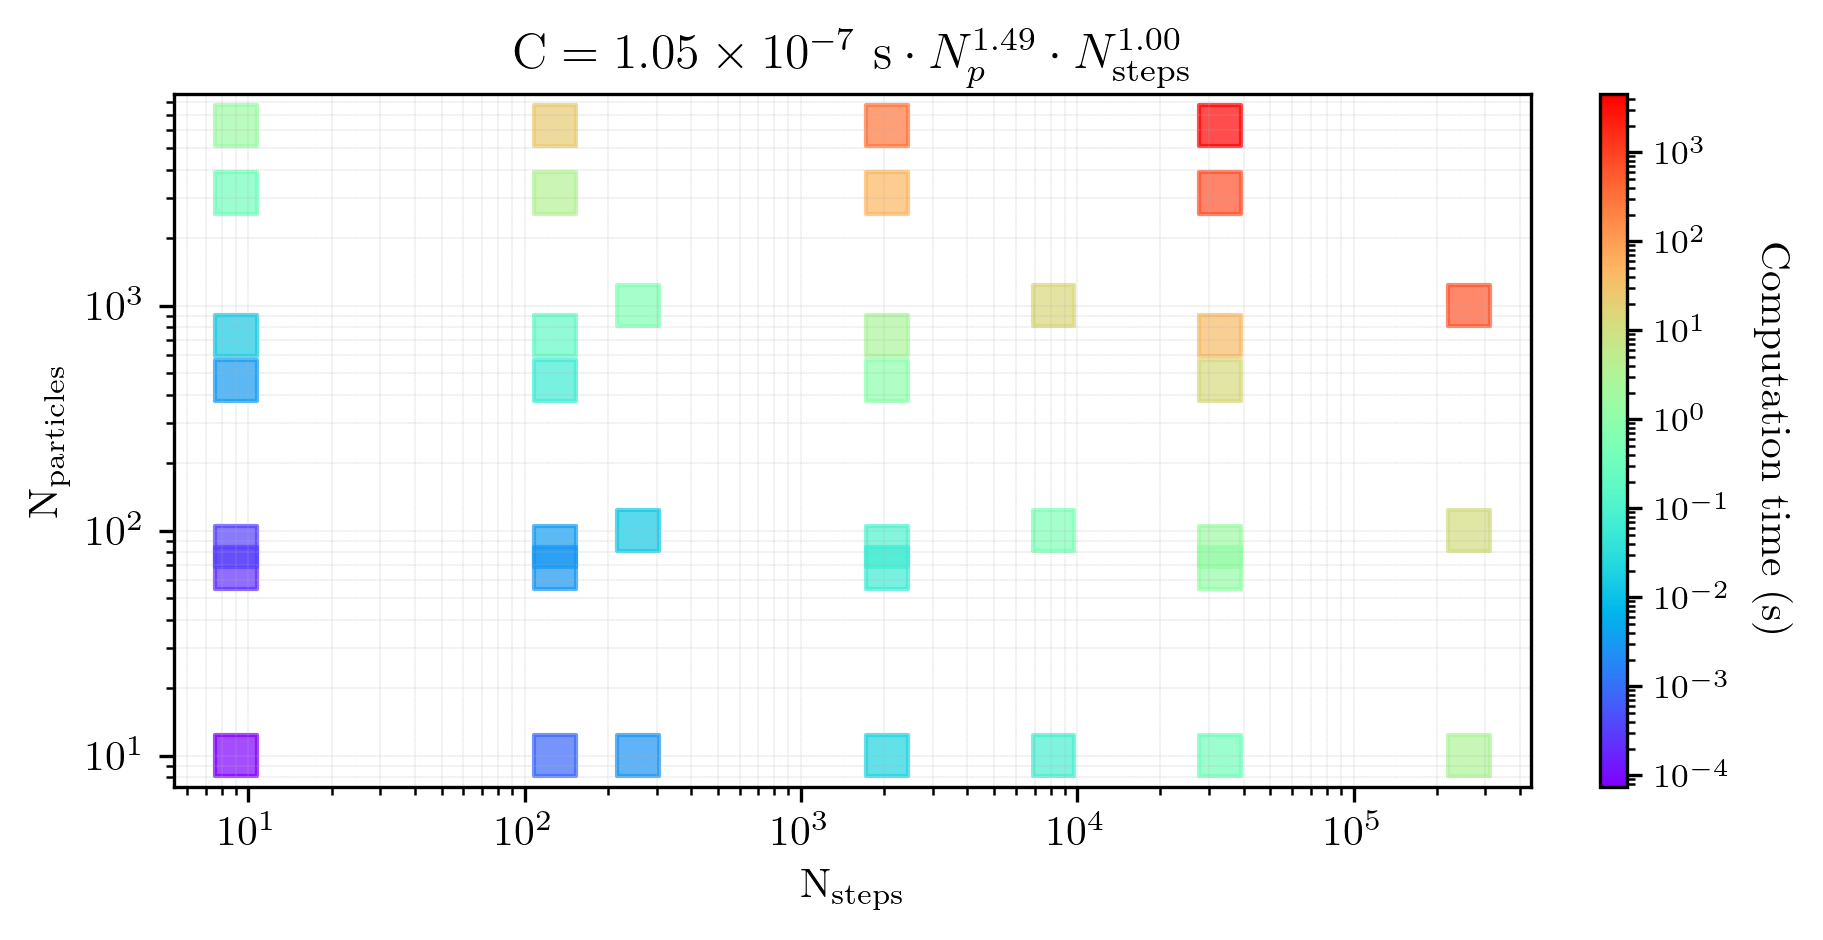
\includegraphics[width=\linewidth]{images/NumericalErrorComputationTimeScalingForStreams.png}
            \caption{How the computation scale time scales with the number of particles and the number of steps taken.}
            \label{fig:NumericalErrorComputationTimeScalingForStreams}
        \end{figure}

        Putting Fig.~\ref{fig:NumericalErrorStreamRetraceEnergyConservation} and Fig.~\ref{fig:NumericalErrorComputationTimeScalingForStreams} together, we get some good estimate for how long it completes to run these simulations. If we want all simualtions to have error better relative error on the retraced conservation of energy than about 10$^{-3}$, then we must pick time steps that are smaller than about 1/20 of the dynamical time. With this criteria selected, we can compute the number of time steps necessary for each globular cluster, which is a function of it's internal dynamical time. By doing so, I find that the fastest cluster can be computed in $\sim$~30~minutes. The median computation time is $\sim$17~hours. The largest computation time was $\sim$~5~days. The total CPU time for the whole catalog is $\sim$~194~days. 

        \subsubsection{A note on non-symplectic integration}

        During the writing of this thesis, I discovered a bug in my code that affected the integration scheme. Specifically, the error concerned the way I handled the host orbit during the integration of the star particles. In earlier implementations, I would integrate the orbit of the host using the same time step that I used later to integrate the orbits of the star particles. However, this approach violated the structure of the leapfrog integration scheme.

        In Hamiltonian integration, it is essential that the drift and kick steps alternate in a consistent manner. Since I implemented a \textit{drift}-\textit{kick}-\textit{drift} (DKD) scheme, the kicks occur at the midpoint of each time step, meaning that forces should be evaluated at intermediate positions. Previously, I erroneously computed the relative position vector as
        \[
        \Delta \vec{r}_i = \vec{r}_{p,i+1/2} - \vec{r}_\mathrm{GC,i},
        \]
        instead of the correct expression:
        \[
        \Delta \vec{r}_i = \vec{r}_{p,i+1/2} - \vec{r}_\mathrm{GC,i+1/2}.
        \]

        This mistake appeared in both \citet{2023A&A...673A..44F} and \citet{2025arXiv250203941F}. Does this invalidate our results? To assess the impact, we can compare Figs.~\ref{fig:NumericalErrorStreamRetrace_Pal5_Nsteps_32768_stepsPerTau_420} and \ref{fig:NumericalErrorStreamRetrace_NGC6171_Nsteps_1048576_stepsPerTau_311}. In Fig.~\ref{fig:NumericalErrorStreamRetrace_Pal5_Nsteps_32768_stepsPerTau_420}, the same retracing experiment was performed, but using the flawed integration: the host orbit was only provided at the same grid points as the stream. In the left panel, we see that the globular cluster does not perfectly re-coalesce when integrating backward in time, but the result is not catastrophic. Physically, we do not expect this process to be perfectly time-reversible; however, such irreversibility should ideally arise from physical modeling, not from numerical artifacts.

        We also observe that the distribution of the relative error in energy conservation is nearly identical between the retraced and the original stream. In any case, once the stars move beyond the Jacobi radius, their dynamics are dominated by the galactic potential. Since this potential was integrated correctly and symplectically, the orbits of stars outside the cluster remain reliable and physically meaningful.

        \begin{figure}
            \centering
            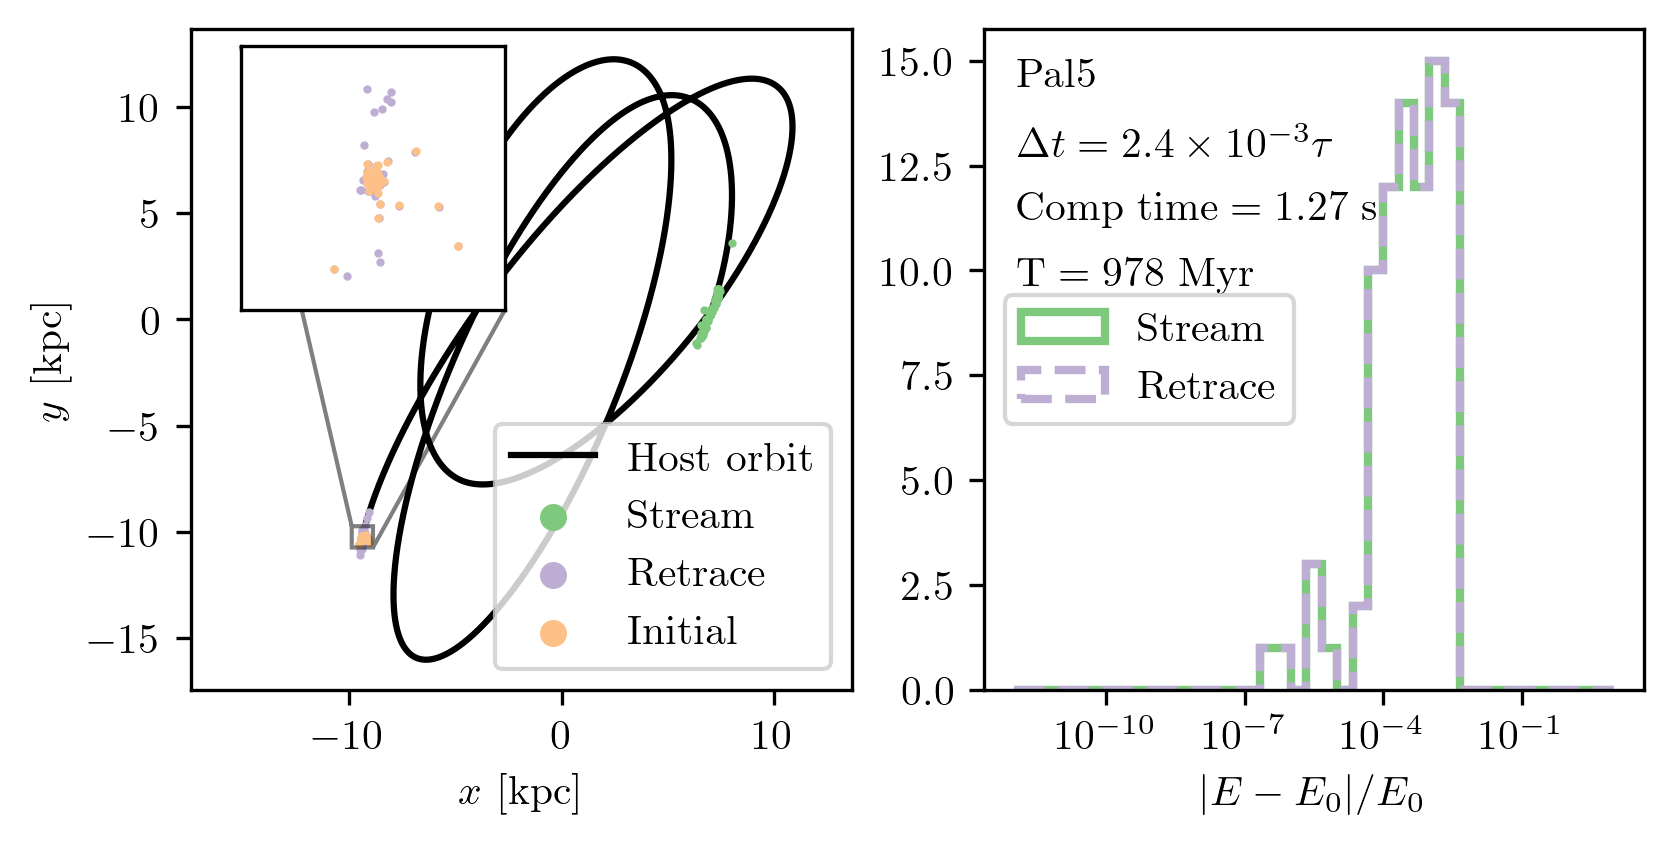
\includegraphics[width=\linewidth]{images/NumericalErrorStreamRetrace_Pal5_Nsteps_32768_stepsPerTau_420.png}
            \caption{An illustration of how an incorrect integration scheme breaks time reversibility. The center of mass of Palomar~5 was integrated backward in time by 1~$\mathrm{s}~\frac{\mathrm{kpc}}{\mathrm{km}}$. A Plummer sphere with 464 particles was sampled around this position (labeled “Initial”), then integrated forward to produce the “Stream.” The right panel shows the distribution of relative energy error. The stream was then integrated backward in time by the same amount, resulting in the “Retrace” configuration. The time step was chosen as a fraction of the internal dynamical timescale, $\tau$.}
            \label{fig:NumericalErrorStreamRetrace_Pal5_Nsteps_32768_stepsPerTau_420}
        \end{figure}

        As a result of this discovery, I updated the \texttt{tstrippy} code to warn users if the host orbit is not sampled at $2N + 1$ points, where $N$ is the number of integration steps. While the flawed implementation breaks strict symplecticity for the internal cluster dynamics, the leapfrog integration for the globular cluster orbits was still used correctly. This ensures that the cluster center of mass returns to its present-day sky position and that stars outside the cluster follow accurate galactic orbits. Ultimately, the simplification of using a static Plummer sphere—whose mass and size remain fixed—is a greater limitation than this particular numerical error.

        Lastly, I discovered this error while writing about the Forest-Ruth integration method. To implement this scheme correctly, I would need to know the position of the globular cluster’s center of mass at four intermediate points across two time steps, with the spacing determined by the coefficients in Table~\ref{tab:forest_ruth_coeffs}. This would require either storing additional mini-time-step data or interpolating the globular cluster's trajectory between saved snapshots. Both options would necessitate a substantial refactoring of the code or an impractical increase in memory usage per orbit. Given the results shown in Fig.~\ref{fig:numericalErrorMeanEnergyErrorRuthForestLeapFrog}, the gain in accuracy does not justify the computational cost.

    \subsection{The Galactic Bar}

        \subsubsection{The globular cluster population}


        \subsubsection{Stream generation in a barred potential}


\section{Tstrippy}

    \begin{itemize}
        \item How does \texttt{tstrippy} actually work?
        \item f2py? 
        \item setuptools $\rightarrow$ meson 
        \item incompatbile with old mac processors and being blocked at numpy 1.23 until the meson migration 
        \item what about other codes on the market? Why did I decide to write this code? 
    \end{itemize}

    \citet{2018ComAC...5....2V} talks about a series of papers between a larger collaboration of people who specialize in collisional dynamics and who have performed a series of workshops together. The introduction stated that the collaboration wants to tackle many open questions regarding stellar clusters and build the necessary codes to interprete the future large quantity of data that was destined to come. It has now come since the review was 2018. An interesting point was that in general globular clusters are approximated as being orderless, i.e. isotropic but order does present itself within these stelalr systems. Another large problem is no one knows what a good set of initial conditiosn is. Unresolved binaries pose a problem because you can overestiamte the total mass of the system. If I talk about this review, I should probably discuss some of the results from the papers that is builds on or at least their techinques.

    The MODEST review led me to discover AMUSE, which is an framework for integrating various astrophysical codes for solving 4 types of problems: gravitational dynamics, radiative transfer, hydrodynamics, and stellar evolution. The codes are written by the community and are interfaced together with Amuse. The user end is python. I have spent some time reading the book, which is instructive and well written. Steve McMillian is one of the authors. The code has a large support on GitHub and is still being developped. I have had trouble trying to install the code. It seems as though their documentation is incoherrent. At one place, it said `pip' is the easiest way to install. It didn't work. In another place, I was instructed to install a zipped up tarball. The setup failed becuase it expected there to be a .git file in the directory. I successfully downloaded the code by cloneing the repository, despite the fact that this was not recommended. I can use some aspects of the code but not all of them. For instance, my memory tells me that about 80\% of the test suite passed, thus many scripts failed. This was when I only installed the frame-work, which was advised since installing the whole package is huge and unnecessary since I am not solving all astrophysical problems. However, I wasn't able to use one of the gravity solvers that was presented in the textbook `AstrophysicalRecipes The art of AMUSE'. The install still has some codes that failed for instance: amuse-adaptb, amuse-hermite-grx, amuse-mi6. However, I'm hoping that this isn't necessary. I want to educate myself and make some examples. 

    Installing other codes and figuring out their functionalities to me has never been trivial. This is similar to galpy when I tried to figure out particle spray method and got less than good results. Agama also confused me a bit. The main point is that for each package, at the end of the day I decided that it was easier and better if I solved the problem myself with my own code. Because, even with the other packages, I know that they can be used to solve other astrophysical problems and it wasn't clear to me how to make the codes solve my specific set of of the restricted three body problems in a potential with other perturbers flying around. 

    In this search, I also discovered another review called \textit{Computational methods for collisional stellar systems} by Spurzem and Kamlah 2023. It is also interesting and instructive. I found it insightful when they called NBody an industry. I think the story of GRAPE and Makino is really interesting, how he build dedicated hardware for the nbody problem which were great for 10 years but were quickly replaced by GPU technology. 
    \begin{itemize}
        \item f2py, and why did we choose to use Fortran? 
        \item Bovy's guide for making a public python package
        \item migrating going from setuptools to meson
        \item a brief overview of how it works. 
        \item how I can either save orbits or snapshots
    \end{itemize}


        \subsection{parallelization}
            Since all star-particles are independent from one another, they can be parallelized. This is \textit{data}-parallelization, where the same job is being performed but the input data is changed. This is a much easier paradigm compared to \textit{task}-parallelization different processors do different things to do the data and may need to communicate with one another. In this experiment, since I am simulating the whole globular cluster catalog and sampling the orbital uncertainties with monte-carlo, as explained in Chapter~5, I often times parallelize over different clusters. 
            
            
            Here is an example slurm script that I use to submit all the jobs: XXX
            
            However, if I want to accelerate one particular computation, then I must split the number of particles into batches. If I run small simulations on my personal computer, I can take the total number of particles and divide by the number of desired batches. Usually, I divide into the number of processors that I am going to use. $N_\mathrm{per~batch}=N_p//N_\mathrm{batches}$. However, I need to integer divide because the number of particles needs to be an integer. Then, with the last batch, I add the remaining particles, which is $N_\mathrm{left over} = N_p - N_\mathrm{batches} \times N_\mathrm{per~batch}$. 



